\documentclass{article}
\usepackage[utf8]{inputenc}
\usepackage{mathtools}
\usepackage{amssymb}
\usepackage{amsmath}
\usepackage{listings}
\usepackage{braket}
\usepackage[toc,page]{appendix}

%%%THEOREM (ETC) ENVIRONMENTS
\newtheorem{definition}{Definition}
\newtheorem{claim}{Claim}
\newtheorem{conjecture}{Conjecture}
\newtheorem{corollary}{Corollary}
\newtheorem{example}{Example}
\newtheorem{problem}{Problem}
\newtheorem{idea}{Idea} 

\usepackage{proof}
\newtheorem{theorem}{Theorem}

\newtheorem{lemma}[theorem]{Lemma}
\newtheorem{proposition}[theorem]{Proposition}

\newenvironment{proof}[1][Proof]{\begin{trivlist}
		\item[\hskip \labelsep {\bfseries #1}]}{\begin{flushright}$\blacksquare$\end{flushright} \end{trivlist}}
\newenvironment{remark}[1][Remark]{\begin{trivlist}
		\item[\hskip \labelsep {\bfseries #1}]}{\end{trivlist}}

\newcommand{\cat}{\mathcal{C}}
\newcommand{\Tau}{\mathrm{T}}
\newcommand{\ham}{\mathcal{H}}
\title{Hopf Algebras in Quantum Computation}
\author{Giovanni de Felice}
\date{April 2017}

%%%TIKZ:
\usepackage{tikz,pgfplots}
\usetikzlibrary{shapes.geometric}
\usetikzlibrary{trees, patterns}
\usetikzlibrary{positioning}
\usepackage{tikz,ifthen,calc}
\usepackage{tkz-euclide}
\usetikzlibrary{shapes,snakes}
\usetikzlibrary{calc,intersections, fit, knots, hobby, positioning, patterns}
\usepackage{braids}

%%%categorical diagrams:
\tikzset{
	buffer/.style={
		draw,
		shape border rotate=180,
		regular polygon,
		regular polygon sides=3,
		node distance=2cm,
		minimum height=4em
	}
}
\tikzstyle{arr}=[markings,mark=at position 0.5 with {\arrow{<}}]
%%%HOPF ALGEBRAS:
\newcommand{\mult}{
	
\begin{tikzpicture}[scale=0.2, black/.style={scale=0.5,draw,shape=circle,fill=black}]
	\node[black] (0) at (0, 0) {};
	\draw (1,-1) to (0);
	\draw (-1,-1) to (0);
	\draw (0) to (0,1);
	\end{tikzpicture}
}
\newcommand{\unit}{
	
\begin{tikzpicture}[scale=0.2, black/.style={scale=0.5,draw,shape=circle,fill=black}]
	\node[black] (0) at (0, 0) {};
	\draw (0) to (0,1);
	\end{tikzpicture}
}
\newcommand{\comult}{
	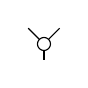
\begin{tikzpicture}[scale=0.2, black/.style={scale=0.5,draw,shape=circle,fill=white}]
	\node[black] (0) at (0, 0) {};
	\draw (1,1) to (0);
	\draw (-1,1) to (0);
	\draw (0) to (0,-1);
	\end{tikzpicture}
}

\newcommand{\counit}{
	\begin{tikzpicture}[scale=0.2, black/.style={scale=0.5,draw,shape=circle,fill=white}]
	\node[black] (0) at (0, 0) {};
	\draw (0) to (0,-1);
	\end{tikzpicture}
}

\newcommand{\antipode}{
	\begin{tikzpicture}[scale=0.2, black/.style={scale=0.5,draw,regular polygon,
		regular polygon sides=4,fill=white}]
	\node[scale=0.5, black] (0) at (0, 0) {$S$};
	\draw (0) to (0,-1);
	\draw (0) to (0,1);
	\end{tikzpicture}
}

\newcommand{\associativity}{
	\begin{equation}
	\begin{gathered}
	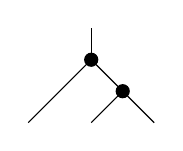
\begin{tikzpicture}[scale=0.8]
	\node[scale=0.5,draw,circle,fill=black] (0) at (0,0.5) {};
	\node[scale=0.5,draw,circle,fill=black] (1) at (0.5,0) {};
	\draw (0) to (1);
	\draw (-1,-0.5) to (0);
	\draw (0,-0.5) to (1);
	\draw (1,-0.5) to (1);
	\draw (0) to (0,1);
	\end{tikzpicture}
	\end{gathered}
	\, = \,
	\begin{gathered}
	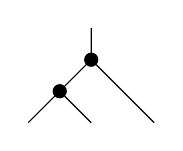
\begin{tikzpicture}[scale=0.8]
	\node[scale=0.5,draw,circle,fill=black] (0) at (0.5,0.5) {};
	\node[scale=0.5,draw,circle,fill=black] (1) at (0,0) {};
	\draw (0) to (1);
	\draw (-0.5,-0.5) to (1);
	\draw (0.5,-0.5) to (1);
	\draw (1.5,-0.5) to (0);
	\draw (0) to (0.5,1);
	\end{tikzpicture}
	\end{gathered}
	\end{equation}
}
\newcommand{\unitlaw}{
	\begin{equation}
	\begin{gathered}
	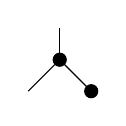
\begin{tikzpicture}[scale=0.8]
	\node[scale=0.5,draw,circle,fill=black] (0) at (0,0.5) {};
	\node[scale=0.5,draw,circle,fill=black] (1) at (0.5,0) {};
	\draw (0) to (1);
	\draw (-0.5,0) to (0);
	\draw (0) to (0,1);
	\end{tikzpicture}
	\end{gathered}
	\, = \,
	\begin{gathered}
	\begin{tikzpicture}[scale=0.8]
	\draw (0,0) to (0,1);
	\end{tikzpicture}
	\end{gathered}
	\, = \,
	\begin{gathered}
	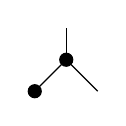
\begin{tikzpicture}[scale=0.8]
	\node[scale=0.5,draw,circle,fill=black] (0) at (0,0.5) {};
	\node[scale=0.5,draw,circle,fill=black] (1) at (-0.5,0) {};
	\draw (0) to (1);
	\draw (0.5,0) to (0);
	\draw (0) to (0,1);
	\end{tikzpicture}
	\end{gathered}
	\end{equation}
}
\newcommand{\coassociativity}{
	\begin{equation}
	\begin{gathered}
	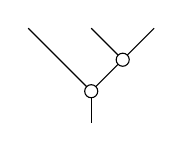
\begin{tikzpicture}[scale=0.8]
	\node[scale=0.5,draw,circle,fill=white] (0) at (0,-0.5) {};
	\node[scale=0.5,draw,circle,fill=white] (1) at (0.5,0) {};
	\draw (0) to (1);
	\draw (-1,0.5) to (0);
	\draw (0,0.5) to (1);
	\draw (1,0.5) to (1);
	\draw (0) to (0,-1);
	\end{tikzpicture}
	\end{gathered}
	\, = \,
	\begin{gathered}
	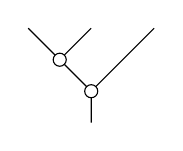
\begin{tikzpicture}[scale=0.8]
	\node[scale=0.5,draw,circle,fill=white] (0) at (0.5,-0.5) {};
	\node[scale=0.5,draw,circle,fill=white] (1) at (0,0) {};
	\draw (0) to (1);
	\draw (-0.5,0.5) to (1);
	\draw (0.5,0.5) to (1);
	\draw (1.5,0.5) to (0);
	\draw (0) to (0.5,-1);
	\end{tikzpicture}
	\end{gathered}
	\end{equation}
}
\newcommand{\counitlaw}{
	\begin{equation}
	\begin{gathered}
	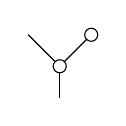
\begin{tikzpicture}[scale=0.8]
	\node[scale=0.5,draw,circle,fill=white] (0) at (0,-0.5) {};
	\node[scale=0.5,draw,circle,fill=white] (1) at (0.5,0) {};
	\draw (0) to (1);
	\draw (-0.5,0) to (0);
	\draw (0) to (0,-1);
	\end{tikzpicture}
	\end{gathered}
	\, = \,
	\begin{gathered}
	\begin{tikzpicture}[scale=0.8]
	\draw (0,0) to (0,1);
	\end{tikzpicture}
	\end{gathered}
	\, = \,
	\begin{gathered}
	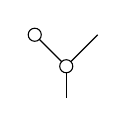
\begin{tikzpicture}[scale=0.8]
	\node[scale=0.5,draw,circle,fill=white] (0) at (0,-0.5) {};
	\node[scale=0.5,draw,circle,fill=white] (1) at (-0.5,0) {};
	\draw (0) to (1);
	\draw (0.5,0) to (0);
	\draw (0) to (0,-1);
	\end{tikzpicture}
	\end{gathered}
	\end{equation}
}

\newcommand{\bialgebralaw}{
	\begin{equation}
	\begin{gathered}
	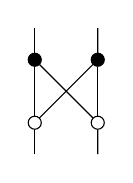
\begin{tikzpicture}[scale=0.8]
	\node[scale=0.5,draw,circle,fill=white] (0) at (0,0) {};
	\node[scale=0.5,draw,circle,fill=white] (1) at (1,0) {};
	\node[scale=0.5,draw,circle,fill=black] (2) at (0,1) {};
	\node[scale=0.5,draw,circle,fill=black] (3) at (1,1) {};
	\draw (0) to (2);
	\draw (0) to (3);
	\draw (1) to (2);
	\draw (1) to (3);
	\draw (0,-0.5) to (0);
	\draw (1,-0.5) to (1);
	\draw (0,1.5) to (2);
	\draw (1,1.5) to (3);
	\end{tikzpicture}
	\end{gathered}
	\, = \,
	\begin{gathered}
	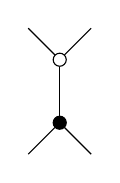
\begin{tikzpicture}[scale=0.8]
	\node[scale=0.5,draw,circle,fill=black] (0) at (0.5,0) {};
	\node[scale=0.5,draw,circle,fill=white] (1) at (0.5,1) {};
	\draw (0) to (1);
	\draw (0,-0.5) to (0);
	\draw (1,-0.5) to (0);
	\draw (0,1.5) to (1);
	\draw (1,1.5) to (1);
	\end{tikzpicture}
	\end{gathered}
	\end{equation}
}
\newcommand{\copylaw}{
	\begin{equation}
	\begin{gathered}
	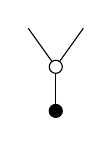
\begin{tikzpicture}[scale=0.7, squr/.style={scale=0.5,draw,regular polygon,
		regular polygon sides=4,fill=white}, black/.style={scale=0.5,draw,shape=circle,fill=black}, whit/.style={scale=0.5,draw,shape=circle,fill=white}]
	\node[black] (0) at (0, 0) {};
	\node[whit] (1) at  (0, 0.8) {};
	\draw (0) to (1);
	\draw (1) to (0.5,1.5);
	\draw (1) to (-0.5,1.5);
	\end{tikzpicture}
	\end{gathered}
	\, = \,
	\begin{gathered}
	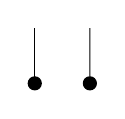
\begin{tikzpicture}[scale=0.7, black/.style={scale=0.5,draw,shape=circle,fill=black}]
	\node[black] (0) at (0,0) {};
	\node[black] (1) at (1,0) {};
	\draw (0) to (0,1);
	\draw (1) to (1,1);
	\end{tikzpicture}
	\end{gathered}
	\end{equation}
}
\newcommand{\cocopylaw}{
	\begin{equation}
	\begin{gathered}
	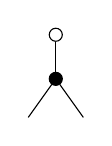
\begin{tikzpicture}[scale=0.7, squr/.style={scale=0.5,draw,regular polygon,
		regular polygon sides=4,fill=white}, black/.style={scale=0.5,draw,shape=circle,fill=black}, whit/.style={scale=0.5,draw,shape=circle,fill=white}]
	\node[whit] (0) at (0, 0) {};
	\node[black] (1) at  (0, -0.8) {};
	\draw (0) to (1);
	\draw (1) to (0.5,-1.5);
	\draw (1) to (-0.5,-1.5);
	\end{tikzpicture}
	\end{gathered}
	\, = \,
	\begin{gathered}
	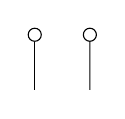
\begin{tikzpicture}[scale=0.7, black/.style={scale=0.5,draw,shape=circle,fill=white}]
	\node[black] (0) at (0,0) {};
	\node[black] (1) at (1,0) {};
	\draw (0) to (0,-1);
	\draw (1) to (1,-1);
	\end{tikzpicture}
	\end{gathered}
	\end{equation}
}
\newcommand{\hopflaw}{
	\begin{equation}
	\begin{gathered}
	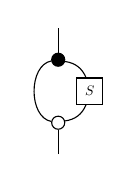
\begin{tikzpicture}[scale=0.8, squr/.style={scale=0.5,draw,regular polygon,
		regular polygon sides=4,fill=white}]
	\node[scale=0.5,draw,circle,fill=white] (0) at (0,0) {};
	\node[scale=0.5,draw,circle,fill=black] (1) at (0,1) {};
	\node[squr] (2) at (0.5,0.5) {$S$};
	\draw[bend left=80] (0) to (1);
	\draw[bend right] (0) to (2);
	\draw[bend right] (2) to (1);
	\draw (0,-0.5) to (0);
	\draw (0,1.5) to (1);
	\end{tikzpicture}
	\end{gathered}
	\, = \,
	\begin{gathered}
	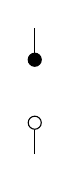
\begin{tikzpicture}[scale=0.8, squr/.style={draw,regular polygon,
		regular polygon sides=4,fill=white}]
	\node[scale=0.5,draw,circle,fill=white] (0) at (0,0) {};
	\node[scale=0.5,draw,circle,fill=black] (1) at (0,1) {};
	\draw (0,-0.5) to (0);
	\draw (0,1.5) to (1);
	\end{tikzpicture}
	\end{gathered}
	\, = \,
	\begin{gathered}
	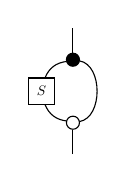
\begin{tikzpicture}[scale=0.8, squr/.style={scale=0.5,draw,regular polygon,
		regular polygon sides=4,fill=white}]
	\node[scale=0.5,draw,circle,fill=white] (0) at (0,0) {};
	\node[scale=0.5,draw,circle,fill=black] (1) at (0,1) {};
	\node[squr] (2) at (-0.5,0.5) {$S$};
	\draw[bend right=80] (0) to (1);
	\draw[bend left] (0) to (2);
	\draw[bend left] (2) to (1);
	\draw (0,-0.5) to (0);
	\draw (0,1.5) to (1);
	\end{tikzpicture}
	\end{gathered}
	\end{equation}
}
\newcommand{\modulelaw}{
	\begin{equation}
	\begin{gathered}
	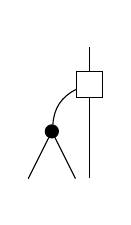
\begin{tikzpicture}[scale=0.6, squr/.style={draw,regular polygon,
		regular polygon sides=4,fill=white}, black/.style={scale=0.5,draw,shape=circle,fill=black}]
	\node (0) at (0, -2.2) {};
	\node[squr] (1) at (0, 0) {};
	\node (2) at (0, 1) {};
	\node[black] (3) at (-0.8, -1) {};
	\draw (0) to (1);
	\draw (1) to (2);
	\draw[bend left] (3) to (1);
	\draw (-1.3, -2) to (3);
	\draw (-0.3, -2) to (3);
	\end{tikzpicture}
	\end{gathered}
	\, = \,
	\begin{gathered}
	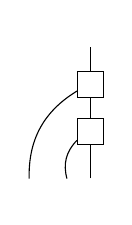
\begin{tikzpicture}[scale=0.6, squr/.style={draw,regular polygon,
		regular polygon sides=4,fill=white}, black/.style={draw,shape=circle,fill=black}]
	\node (0) at (0, -2.2) {};
	\node[squr] (1) at (0, 0) {};
	\node (2) at (0, 1) {};
	\node[squr] (3) at (0, -1) {};
	\draw (0) to (3);
	\draw (3) to (1);
	\draw (1) to (2);
	\draw (3) to (1);
	\draw[bend left] (-1.3, -2) to (1);
	\draw[bend left] (-0.5, -2) to (3);
	\end{tikzpicture}
	\end{gathered}
	\end{equation}
}
\newcommand{\comodulelaw}{
	\begin{equation}
	\begin{gathered}
	\begin{tikzpicture}[scale=0.6, squr/.style={draw,regular polygon,
		regular polygon sides=4,fill=white}, black/.style={scale=0.5,draw,shape=circle,fill=white}]
	\node (0) at (0, 2.2) {};
	\node[squr] (1) at (0, 0) {};
	\node (2) at (0, -2) {};
	\node[black] (3) at (-0.8, 1) {};
	\draw (0) to (1);
	\draw (1) to (2);
	\draw[bend right] (3) to (1);
	\draw (-1.3, 2) to (3);
	\draw (-0.3, 2) to (3);
	\end{tikzpicture}
	\end{gathered}
	\, = \,
	\begin{gathered}
	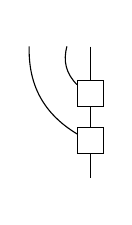
\begin{tikzpicture}[scale=0.6, squr/.style={draw,regular polygon,
		regular polygon sides=4,fill=white}, black/.style={draw,shape=circle,fill=black}]
	\node (0) at (0, 2.2) {};
	\node[squr] (1) at (0, 0) {};
	\node (2) at (0, -1) {};
	\node[squr] (3) at (0, 1) {};
	\draw (0) to (3);
	\draw (3) to (1);
	\draw (1) to (2);
	\draw (3) to (1);
	\draw[bend right] (-1.3, 2) to (1);
	\draw[bend right] (-0.5, 2) to (3);
	\end{tikzpicture}
	\end{gathered}
	\end{equation}
}
\newcommand{\intertwinerlaw}{
	\begin{equation}
	\begin{gathered}
	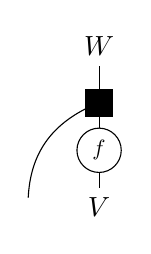
\begin{tikzpicture}[scale=0.6, squr/.style={draw,regular polygon,
		regular polygon sides=4,fill=black}]
	\node (0) at (0, -2.2) {$V$};
	\node[squr] (1) at (0, 0) {};
	\node (2) at (0, 1.2) {$W$};
	\node[scale=0.8,draw,circle] (3) at (0, -1) {$f$};
	\draw (0) to (3);
	\draw (3) to (1);
	\draw (1) to (2);
	\draw (3) to (1);
	\draw[bend left] (-1.5, -2) to (1);
	\end{tikzpicture}	
	\end{gathered}
	\, = \,
	\begin{gathered}
	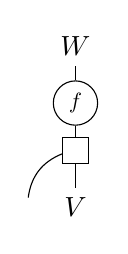
\begin{tikzpicture}[scale=0.6, squr/.style={draw,regular polygon,
		regular polygon sides=4,fill=white}]
	\node (0) at (0, -2.2) {$V$};
	\node[scale=0.8,draw,circle] (1) at (0, 0) {$f$};
	\node (2) at (0, 1.2) {$W$};
	\node[squr] (3) at (0, -1) {};
	\draw (0) to (3);
	\draw (3) to (1);
	\draw (1) to (2);
	\draw (3) to (1);
	\draw[bend left] (-1, -2) to (3);
	\end{tikzpicture}	
	\end{gathered}
	\end{equation}
}
\newcommand{\symAB}{
	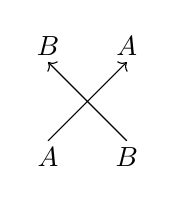
\begin{tikzpicture}[decoration={markings,mark=at position 0.5 with {\arrow{>}}}]
	\node (0) at (-0.5, -0.7) {$A$};
	\node (0) at (-0.5, 0.7) {$B$};
	\node (1) at (0.5, -0.7) {$B$};
	\node (1) at (0.5, 0.7) {$A$};
	\draw [->] (-0.5, -0.5) to (0.5, 0.5);
	\draw [->] (0.5, -0.5) to (-0.5, 0.5);
	\end{tikzpicture}
}

\newcommand{\symequation}{
	\begin{equation*}
	\begin{gathered}
	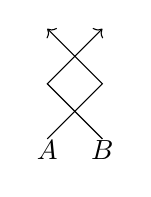
\begin{tikzpicture}[scale=0.7]
	\node (0) at (-1, -1.2) {$A$};
	\node (0) at (0, -1.2) {$B$};
	\draw [->] (-1, -1)--(0,0)--(-1,1);
	\draw [->] (0, -1)--(-1,0)--(0,1);
	\end{tikzpicture}
	\end{gathered}
	\, = \,
	\begin{gathered}
	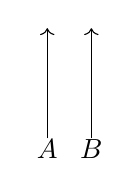
\begin{tikzpicture}[scale=0.7]
	\node (0) at (-0.8, -1.2) {$A$};
	\node (0) at (0, -1.2) {$B$};
	\draw [->] (-0.8, -1)--(-0.8,1);
	\draw [->] (0, -1)--(0,1);
	\end{tikzpicture}
	\end{gathered}
	\end{equation*}
}

\newcommand{\cupA}{	
	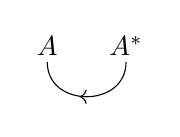
\begin{tikzpicture}[decoration={markings,mark=at position 0.5 with {\arrow{<}}}]
	\node (0) at (0, 0.2) {$A$};
	\node (1) at (1, 0.2) {$A^*$};
	\draw [bend right=90, looseness=1.5, postaction=decorate] (0,0) to (1,0);
	\end{tikzpicture}}

\newcommand{\capA}{	
	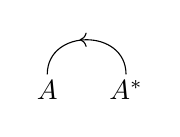
\begin{tikzpicture}[decoration={markings,mark=at position 0.5 with {\arrow{<}}}]
	\node (0) at (0, -0.2) {$A$};
	\node (1) at (1, -0.2) {$A^*$};
	\draw [bend left=90, looseness=1.5, postaction=decorate] (0,0) to (1,0);
	\end{tikzpicture}}

\newcommand{\snake}{
	\begin{equation*}
	\begin{gathered}
	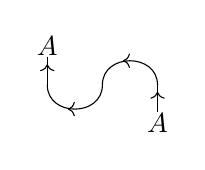
\begin{tikzpicture}[scale=0.7,decoration={markings,mark=at position 0.5 with {\arrow{<}}}]
	\node (0) at (0, 0.7) {$A$};
	\node (4) at (2, -0.7){$A$};
	\draw [bend right=90, looseness=1.5, postaction=decorate] (0, 0) to (1, 0);
	\draw [bend left=90, looseness=1.5, postaction=decorate] (1, 0) to (2, 0);
	\draw [postaction=decorate] (2, 0) to (2, -0.5);
	\draw [postaction=decorate] (0, 0.5) to (0, 0);
	\end{tikzpicture}
	\end{gathered}
	\, = \,
	\begin{gathered}
	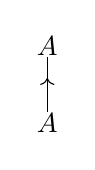
\begin{tikzpicture}[scale=0.7,decoration={markings,mark=at position 0.5 with {\arrow{<}}}]
	\node (0) at (0, 0.7) {$A$};
	\node (4) at (0, -0.7){$A$};
	\draw [postaction=decorate] (0, 0.5) to (0, -0.5);
	\end{tikzpicture}
	\end{gathered}
	\end{equation*}}

\newcommand{\snakestar}{
	\begin{equation*}
	\begin{gathered}
	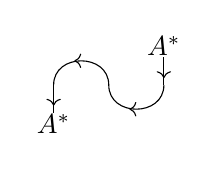
\begin{tikzpicture}[scale=0.7,decoration={markings,mark=at position 0.5 with {\arrow{<}}}]
	\node (0) at (0, -0.7) {$A^*$};
	\node (4) at (2, 0.7){$A^*$};
	\draw [bend left=90, looseness=1.5, postaction=decorate] (0, 0) to (1, 0);
	\draw [bend right=90, looseness=1.5, postaction=decorate] (1, 0) to (2, 0);
	\draw [postaction=decorate] (2, 0) to (2, 0.5);
	\draw [postaction=decorate] (0, -0.5) to (0, 0);
	\end{tikzpicture}
	\end{gathered}
	\, = \,
	\begin{gathered}
	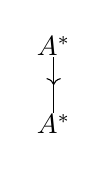
\begin{tikzpicture}[scale=0.7,decoration={markings,mark=at position 0.5 with {\arrow{>}}}]
	\node (0) at (0, 0.7) {$A^*$};
	\node (4) at (0, -0.7){$A^*$};
	\draw [postaction=decorate] (0, 0.5) to (0, -0.5);
	\end{tikzpicture}
	\end{gathered}
	\end{equation*}
}

\newcommand{\fusionijk}{
	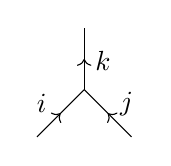
\begin{tikzpicture}[scale=0.6,decoration={markings,mark=at position 0.5 with {\arrow{>}}}]
	\node (0) at (-0.9, -0.3) {$i$};
	\node (1) at (0.9, -0.3) {$j$};
	\node (2) at (0.4, 0.6) {$k$};
	\draw [postaction=decorate] (-1, -1) to(0,0);
	\draw [postaction=decorate] (1,-1) to (0,0);
	\draw [postaction=decorate] (0,0) to (0,1.3);
	\end{tikzpicture}}
%%%%%%%%%%%%%%%%%%%%%%%%%%%%%%%%%%%%%%%%%%%%%%%%%%%%%%%%%%%%%%%%%%%%%%%%%%%%%%%%%%%%%%%%%%%%%%%%%%%%%%%%%%%%%%%%%%%%%%%%%%%%%%%%%%%%%%%%%%%%%%%%%%%%%%%%%%%%%%%%%%%%%%%%%%%%%%%%%%%%


\begin{document}
	
\section{The Algebra of Anyons}
In this section we introduce the physics of Anyons and use the framework developed in the first section to define categorical models for theories of these particles. For an introduction to the physics of anyons consider the foundational paper \cite{Kitaev06} or Simon's notes \cite{Simon16}, for a categorical presentation \cite{Panangaden11} and for a thorough survey of the mathematical aspects of anyons \cite{Rowell17}.\\
In the first section we introduce the physics and make the link with braided fusion categories, in the second part of we will develop the categorical formalism and the third part is dedicated to one result where quantification and categorical constructions play an important role.\\~\\
To understand how anyons arise physically, let us consider $n$ indistinguishable particles evolving in space. The quantum amplitude for a space-time evolution of the system will depend on the topology of the particle word-lines and not on the detailed geometry. This means that isotopic space-time evolution will yield the same amplitude.\\
To formalize the situation suppose we have $n$ indistinguishable particles in $D$ dimensions, the configuration space can be written as:
$$ \mathrm{C}=(\mathbb{R}^{nD}-\Delta)/S_n$$
Where $\Delta$ is the space of coincidences (where at least two of the $n$ particles occupy the same position in $\mathbb{R}^D$). We are quotienting the space by $S_n$ to account for the indistinguishability of the particles (i.e we do not care about the order of the $n$ coordinates in $D$ dimensions). 
Let us fix the starting and endpoint in the configuration space, the space of paths from starting to endpoint $\mathrm{C}$ divides into topologically distinct classes, described by the fundamental group $\pi_1(\mathrm{C})$. These classes account for the different possible exchange statistics of the particles.\\
We can then describe the evolution of the wave function for the system via unitary transformations induced from the element of the fundamental group corresponding to particles word-lines. In mathematical terms this corresponds to a representation of $\pi_1(\mathrm{C})$. \\
If space-time has $D=3+1$ dimensions, the topological class of paths is completely determined by the corresponding permutation of the particles, because there are no knots in $4$ dimensions. Therefore the evolution of the system under particle exchanges will be described by a representation of the symmetric group $S_n$.
In $2+1$ dimensions we have more exotic behaviour, as the paths in configuration space can braid. The time evolution of the wave function is then described by a representation of the braid group on $n$ strands, denoted $B_n$.
\begin{definition}[Braid group]
	The braid group on $n$ strands $B_n$ is the group generated by $\{ \sigma_i: i=1,..,n-1\}$  satisfying the following relations:
	\begin{itemize}
		\item $\sigma_i \sigma_j = \sigma_j \sigma_i$ for $i+1 < j$
		\item $ \sigma_i \sigma_{i+1} \sigma_i = \sigma_{i+1} \sigma_i \sigma_{i+1}$ for $1 < i < n$.
	\end{itemize}
	 The second relation is called Yang-Baxter equation and can be drawn as follows:
\begin{equation}
\begin{gathered}
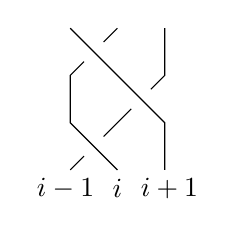
\begin{tikzpicture}[scale=0.6]
\node (0) at (0.5,0.5) {};
\node (1) at (-0.1,-0.4) {$i-1$};
\node (2) at (1,-0.4) {$i$};
\node (3) at (2.1,-0.4) {$i+1$};
\node (4) at (1.5,1.5) {};
\node (5) at (0.5,2.5) {};
\draw (0,0)--(0)--(1,1)--(4)--(2,2)--(2,3);
\draw (1,0)--(0,1)--(0,2)--(5)--(1,3);
\draw (2,0)--(2,1)--(0,3);
\end{tikzpicture}
\end{gathered}
\, = \,
\begin{gathered}
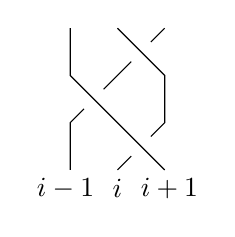
\begin{tikzpicture}[scale=0.6]
\node (0) at (1.5,0.5) {};
\node (1) at (-0.1,-0.4) {$i-1$};
\node (2) at (1,-0.4) {$i$};
\node (3) at (2.1,-0.4) {$i+1$};
\node (4) at (0.5,1.5) {};
\node (5) at (1.5,2.5) {};
\draw (2,0)--(1,1)--(0,2)--(0,3);
\draw (1,0)--(0)--(2,1)--(2,2)--(1,3);
\draw (0,0)--(0,1)--(4)--(5)--(2,3);
\end{tikzpicture}
\end{gathered}
\end{equation}
\end{definition}

\begin{itemize}
	\item Abelian case
\end{itemize}
We say the system is abelian if the wave function lives in a one-dimensional representation of the group of paths in configuration space. In $3+1$ dimensions, this means we have to consider the one-dimensional representations of $S_N$. Note that there are only two possibilities (namely the trivial and the sign representations) corresponding to the two possible types of particle statistics in $3+1$ dimensions (Bose and Fermi statistics respectively).
In $2+1$ dimensions we have many more possibilities as the evolution of the wave function will be described by a one-dimensional representation of the braid group $B_N$. There are infinitely many one dimensional representations of the braid group connecting the fermions and bosons case. These are described by a single parameter $\theta$. Only one parameter because using Yang-Baxter we can show that all $N$ phases have to be the same, also can show $\theta$ has to be a fraction from physical considerations. We obtain abelian anyons.\\
\begin{itemize}
	\item Non-abelian case
\end{itemize}
In the non-abelian case, the wave function lives in a higher-dimensional representation of In $3+1$ dimensions we don't get anything more than bosons and fermions if we also want to consider creation, annihilation (splitting, fusion) of particles (Doplicher-Roberts theorem). 
In $2+1$ dimensions we obtain degeneracy, non-abelian anyons, braidings give all unitaries.\\~\\
In the previous section, we only considered groups of symmetries of a Hamiltonian. In order take topological symmetries of a system into account, we need the more general framework of Hopf Algebras. In particular, as those symmetries arise from braids, we need quasitriangular hopf algebras (or quantum groups) to treat all symmetries on the same level. We will see that the universal $R$-matrix plays an important role in the description of topological dependencies.

\subsection{Models of anyons}
We want to construct a category $\cat$ that models the behaviour of anyons. Ojects of $\cat$ will correspond to quantum systems and morphisms to their possible evolutions, or to the processes we can perform on them.\\
Let us first set a finite set of labels $\{a,b,c...\}$ of distinct particle types, these will be objects of $\cat$. In our theory we must be able to consider many particles at the same time, so $\cat$ must be monoidal \cite{Coecke17}. The unit of the tensor $\mathbf{1}$ corresponds to the vacuum particle type (or "no-particle") and must be within our labels. So for the moment our theory is a monoidal category $\mathcal{C}$ and we can already use the diagrammatic language. A particle of type $a$ evolving trivially in time is denoted:
\begin{center}
\begin{tikzpicture}[scale=0.7, decoration={markings,mark=at position 0.5 with {\arrow{>}}}]
	\node (a) at (0.3,0) {$a$};
	\draw [postaction = decorate] (0,-1) to (0,1);
\end{tikzpicture}
\end{center}
Where we have adopted the convention that time flows upwards.\\
Two particles of types $a$ and $b$ can fuse to a third particle of type $c$. So we have fusion morphisms:
\begin{center}
	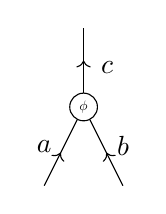
\begin{tikzpicture}[decoration={markings,mark=at position 0.5 with {\arrow{>}}}]
	\node (a) at (-0.5,-0.5) {$a$};
	\node (b) at (0.5,-0.5) {$b$};
	\node (c) at (0.3,0.5) {$c$};
	\node[scale=0.5, draw, circle] (0) at (0,0) {$\phi$};
	\draw [postaction = decorate] (-0.5,-1) to (0);
	\draw [postaction = decorate] (0.5,-1) to (0);
	\draw [postaction = decorate] (0) to (0,1);
	\end{tikzpicture}
\end{center}
Similarly a particle $c$ can split to give two particles $a$ and $b$. And $\cat$ contains splitting morphism:
\begin{center}
	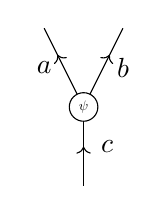
\begin{tikzpicture}[decoration={markings,mark=at position 0.5 with {\arrow{<}}}]
	\node (a) at (-0.5,0.5) {$a$};
	\node (b) at (0.5,0.5) {$b$};
	\node (c) at (0.3,-0.5) {$c$};
	\node[scale=0.5, draw, circle] (0) at (0,0) {$\psi$};
	\draw [postaction = decorate] (-0.5,1) to (0);
	\draw [postaction = decorate] (0.5,1) to (0);
	\draw [postaction = decorate] (0) to (0,-1);
	\end{tikzpicture}
\end{center}
Any particle $a$ in quantum physics comes with its antiparticle $a^*$ which we can picture as a particle of type $a$ travelling backwards in time.
\begin{center}
	\begin{tikzpicture}[scale=0.7, decoration={markings,mark=at position 0.5 with {\arrow{<}}}]
	\node (a) at (0.3,0) {$a$};
	\draw [postaction = decorate] (0,-1) to (0,1);
	\end{tikzpicture}
\end{center}
It has the property of fusing to the vacuum when it encounters $a$. Dually the vacuum can yield a particle-antiparticle pair, so we have cups and caps morphisms
\begin{center}
	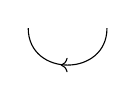
\begin{tikzpicture}[decoration={markings,mark=at position 0.5 with {\arrow{<}}}]
	\draw [bend right=90, looseness=1.6, postaction = decorate] (-0.5,0) to (0.5,0);
	\end{tikzpicture}
	\quad
	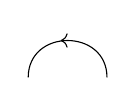
\begin{tikzpicture}[decoration={markings,mark=at position 0.5 with {\arrow{<}}}]
	\draw [bend left=90, looseness=1.6, postaction = decorate] (-0.5,0) to (0.5,0);
	\end{tikzpicture}
\end{center}
Categorically this corresponds to a rigid structure on $\cat$, we will assume it is a well behaved category i.e it is spherical and $1^*=1$. So we can define the quantum numbers for each particle type $a$ to be the following scalar:
\begin{center}
	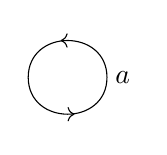
\begin{tikzpicture}[decoration={markings,mark=at position 0.5 with {\arrow{<}}}]
	\node (a) at (0.7,0) {$a$};
	\draw [bend left=90, looseness=1.6, postaction = decorate] (0.5,0) to (-0.5,0);
	\draw [bend left=90, looseness=1.6, postaction = decorate] (-0.5,0) to (0.5,0);
	\end{tikzpicture}
\end{center}
At this point we need to linearise the theory to take superpositions into account. This means we make $\cat$ into a rigid tensor category (see appendix). We have biproducts $\oplus$ to account for superpositions. In order for the fusions to behave well with superpositions we must require that our labels for particle types be simple objects in the category. At this point, our category $\mathcal{C}$ is a spherical fusion category (see appendix) and the fusion rules look like this:
\begin{equation}
a\otimes b \simeq \oplus_c N_{ab}^c c
\end{equation}
Where $N_{ab}^c \in \mathbb{N}$. \\
\begin{definition}
	A fusion category is a finite semisimple k-linear tensor category with two sided duals
\end{definition}
$$dim(\cat) = \sum_i d(X_i)^2$$
$$dim(Rep(H))=dim(H)$$
We still have one question to ask to the theory, what happens when the position of two particles is exchanged? To answer this question the theory must have a braid structure and we obtain a braided fusion category (see section 1). The braid structure determines the long-distance, topological interactions between particles.

\begin{example}
	Suppose we start from a set of labels and define the fusions to form a group. $1$ is the identity particle type, for any particle type $a$, $a^*$ will be its inverse. We have defined the skeleton of a spherical fusion category, which we obtain by linearising, i.e taking a fiber functor to $Hilb$. We obtain the category $Vec_G$, of $G$ graded vector spaces over $\mathbb{C}$.
	The category $Vec_G$ for $G$ a group is a symmetric spherical fusion category. Linearity and tensor are given by the underlying $Vect$ structure, simple objects $V_g$ are one-dimensional and indexed by elements $g \in G$, duality is proved by using the group inverse and fusions are given by the group multiplication.
	$$V_g \otimes V_h \simeq V_{gh}$$
	It is easy to show that $Vec_G \simeq Rep(Func(G))$ where $Func(G)$ is the function algebra on $G$.
	For $G=\mathbb{Z}_2$ we have two irreducible representations $\tau_+$ and $\tau_-$, both one dimensional with the obvious fusion rules given by the cyclic group of order $2$.\\
\end{example}

\begin{remark}
	In the case where the theory is described by the category $RepG$.
	Let us consider the object $V=\mathbb{C}G$ of $RepG$. (Note $V \simeq \oplus_i V_i$ where $V_i$'s are the simple objects.) Simple objects correspond to particle types so the states of $V$ are superpositions of particle types. In the case where $G$ is abelian there is only one way two particles can fuse to a third, so the fusions are deterministic and the irreducible representations will be one dimensional, each corresponding to an element of the group. If $G$ is not abelian, say $a\otimes b \simeq c_1$ and $b \otimes a \simeq c_2$ then taking the representations category defines a 2-dimensional object $c$ spanned by $\{c_1,c_2\}$ which is an irreducible representation of $G$. So from now on we will call particle types the irreducible representations and particles subtypes the elements of the group $G$.  The action of $G$ permutes the basis vectors, multiplying by an element of $G$, but an element of $G$ is precisely a particle subtype and multiplication is fusion. So acting with $g \in G$ on a state $v \in V$ corresponds to fusing a particle of type $g$ with one that is in a superposition $v$ of particle types. The allowed processes are intertwiners which commute with the action and therefore preserve fusions. If the group $G$ is abelian, then the particles are abelian anyons.
\end{remark}

\subsection{Modular categories}


As we have seen in the previous section, braided fusion categories are well suited to describe theories of anyons. These form a big class of categories, some of which are uninteresting from the physical point of view. To distinguish between them we can place braided fusion categories in a spectrum by asking what their symmetric center $Z_2$ is. 

\begin{definition}
	The symmetric center $Z_2(\mathcal{C})$ is the full subcategory of $\mathcal{C}$ defined by:
	$$ obj \, Z_2(\mathcal{C}) = \{ X\in \mathcal{C} : c_{X,Y} \circ c_{Y,X} = id_{Y\otimes X} \quad \forall Y \in \mathcal{C} \} $$
\end{definition}

\begin{definition}
	A braided fusion category is:
	\begin{itemize}
		\item pre-modular if it is spherical,
		\item non-degenerate if $Z_2(\mathcal{C})$ is trivial (i.e it only contains direct sums of the tensor unit as objects, i.e every simple object is isomorphic to the tensor unit)
		\item modular if it is pre-modular and non-degenerate.
	\end{itemize}
\end{definition}

The two opposite ends of this spectrum are symmetric fusion categories on one side (such that $Z_2(\mathcal{C})=\mathcal{C}$) and modular tensor categories (as defined). 
In the first case, we have only symmetric exchange of quantum systems which means all particles in the theory are either bosons or fermions. Such categories are degenerate anyon theories as they exhibit no topological behaviour. Modular categories are really the opposite situation, the theory doesn't contain any bosons or fermions but only non-degenerate anyons (i.e anyons with non-trivial twist factor). Modular categories are very well-behaved theories as we can assign to them the so called modular $S$-matrix which will contain the all the information on fusion rules as well as the braided structure.

\begin{definition}
	Let $\mathcal{C}$ be a spherical braided fusion category and let $I$ be the set of isomorphism classes of simple objects in $\mathcal{C}$. We define $S_{i,j}$ for $i,j \in I$ to be the following:
	\begin{equation}
		S_{i,j} := 
	\end{equation}
\end{definition} 
\begin{definition}
	$T$ matrix given by $tr(B_{X_i,X_i})$
\end{definition}
Then $S$ and $T$ satisfy the same relations as the generators of the modular group $SL(2,\mathbb{Z})$, that's why we call those categories modular.
\begin{definition}
	If $\mathcal{D}$ is a full subcategory of $\mathcal{C}$ can define $D'=\{X \in obj(\mathcal{C}): B_{X,Y} \circ B_{Y,X} = id{X \otimes Y}\}$
\end{definition}
Can define prime modular categories, and if $G$ is simple non-abelian group then $Rep(DG)$ is modular and prime.
\begin{theorem}
	$\mathcal{C}$ is modular iff the $S$-matrix is invertible.
\end{theorem}
\begin{theorem}
	The modular $S$-matrix diagonalises the $N$-matrix.
\end{theorem}
splitting, fusion rules, braided, R,T matrices, modular S matrix.

\begin{example}[Knot invariants]
\end{example}

\subsection{Tannaka duality}
This section is only meant as a motivation for the study of Hopf Algebras and we wont prove the reconstruction theorems, surveys on Tannaka reconstruction are given by \cite{Vercruysse12} and \cite{Joyal91}.\\

Reconstruction results are recipes which produce all the examples of a class of categories (i.e categories with some fixed structure) from simpler mathematical objects.As we have seen in the previous sections, the structure of categories of $H$-modules is induced from the axioms of the Hopf Algebra $H$. It is surprising that Hopf algebras underly most of the categories with this structure.
\begin{theorem}[Tannaka reconstruction]
	\begin{itemize}
		\item Any monoidal category $\cat$ equipped with a fiber functor (i.e a strict monoidal functor) $U: \cat \rightarrow Vect$ is equivalent to $Rep(B)$ where $B$ is a bialgebra.
		\item Any (braided) rigid monoidal category equipped with a fiber functor (here this means strict (braided) rigid monoidal functor) to $Vect$ is equivalent to $Rep(H)$ for some (quasitriangular) hopf algebra $H$.
	\end{itemize}
\end{theorem}

\begin{theorem}
	If $H$ is a finite dimensional, semisimple Hopf algebra the $Rep(D(H))$ is modular.
\end{theorem}

\subsection{The Drinfeld center}
In this section we introduce a general construction that turns braided fusion categories into modular categories, and we show its relationship with the Quantum double construction on a Hopf Algebra introduced in the first chapter.\\
Topological dependencies between objects in fusion categories are captured by the braided structure. Let us fix some definitions before discussing the Drinfeld construction.

\begin{definition}[Half-braiding]
	A half-braiding on some object $X$ in a monoidal category $\cat$ is a natural isomorphism 
	$$ e^X : (-) \otimes X \Rightarrow X \otimes (-)$$
	satisfying: 
	$$e^X_{Y \otimes Z} =( e^X_Z \otimes id_Y) \circ (id_Z \otimes e^X_Y)$$ 
\end{definition}
\begin{definition}[Drinfeld center]
	The braided (Drinfeld) center of a monoidal category $\mathcal{C}$ is the category $Z(\mathcal{C})$ with objects pairs $(X,e^X)$ where $X \in \mathcal{C}$ and $e^X$ is a half-braiding, and with morphisms given by the morphisms of $\mathcal{C}$ which commute with the half-braiding.
\end{definition}
\begin{definition}[Yetter-Drinfeld modules]
	Let $H$ be a bialgebra, the category $\mathcal{D}_{H}^{lr}$ is the category of left-right Yetter-Drinfeld modules where objects are left $H$-modules which are simultaneously right $H$-comodules satisfying the following compatibility condition:
	\begin{equation}
	\begin{gathered}
	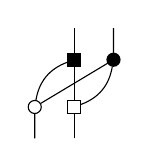
\begin{tikzpicture}[whit/.style={draw,regular polygon,
		regular polygon sides=4,fill=white}, squr/.style={draw,regular polygon,
		regular polygon sides=4,fill=black}]
	\node [scale=0.5, whit] (0) at (0,-0.3) {};
	\node [scale=0.5, squr] (3) at (0,0.3) {};
	\node [scale=0.5, draw, circle, fill=black] (1) at (0.5,0.3) {};
	\node [scale=0.5, draw, circle, fill=white] (2) at (-0.5,-0.3) {};
	\draw (-0.5,-0.7)--(2)--(1)--(0.5,0.7);
	\draw [bend left] (2) to (3);
	\draw [bend right] (0) to (1);
	\draw (0,-0.7)--(0)--(3)--(0,0.7);
	\end{tikzpicture}
	\end{gathered}
	\, = \,
	\begin{gathered}
	\begin{tikzpicture}[whit/.style={draw,regular polygon,
		regular polygon sides=4,fill=white}, squr/.style={draw,regular polygon,
		regular polygon sides=4,fill=black}]
	\node [scale=0.5, whit] (0) at (-0.3,0.3) {};
	\node [scale=0.5, squr] (3) at (0.3,-0.3) {};
	\node [scale=0.5, draw, circle, fill=black] (1) at (0.3,0.5) {};
	\node [scale=0.5, draw, circle, fill=white] (2) at (-0.3,-0.5) {};
	\draw (-0.3,-0.7)--(2)--(1)--(0.3,0.7);
	\draw (2) to (3);
	\draw (0) to (1);
	\draw (-0.3,0.7)--(0);
	\draw[bend right] (0) to (0,0);
	\draw[bend left] (0,0) to (3);
	\draw (3)--(0.3,-0.7);
	\end{tikzpicture}
	\end{gathered}	
	\end{equation}
	where the white box denotes the $H$ coaction and the black box defines the right coaction. Morphisms of $\mathcal{D}_{H}^{lr}$ are both $H$-module and $H$-comodule morphisms. Left-left Yetter-Drinfeld modules are defined in the obvious way and form a category $\mathcal{D}_{H}^{ll}$. The compatibility condition then looks like this:
	\begin{equation}
	\begin{gathered}
	\begin{tikzpicture}[whit/.style={draw,regular polygon,
		regular polygon sides=4,fill=white}, squr/.style={draw,regular polygon,
		regular polygon sides=4,fill=black}]
	\node [scale=0.5, whit] (0) at (0,-0.3) {};
	\node [scale=0.5, squr] (3) at (0,0.3) {};
	\node [scale=0.5, draw, circle, fill=black] (1) at (-0.5,0.3) {};
	\node [scale=0.5, draw, circle, fill=white] (2) at (-0.5,-0.3) {};
	\draw (-0.5,-0.7)--(2)--(1)--(-0.5,0.7);
	\draw (2) to (3);
	\draw (0) to (1);
	\draw (0,-0.7)--(0)--(3)--(0,0.7);
	\end{tikzpicture}
	\end{gathered}
	\, = \,
	\begin{gathered}
	\begin{tikzpicture}[whit/.style={draw,regular polygon,
		regular polygon sides=4,fill=white}, squr/.style={draw,regular polygon,
		regular polygon sides=4,fill=black}]
	\node [scale=0.5, whit] (0) at (0,0.3) {};
	\node [scale=0.5, squr] (3) at (0,-0.3) {};
	\node [scale=0.5, draw, circle, fill=black] (1) at (-0.5,0.5) {};
	\node [scale=0.5, draw, circle, fill=white] (2) at (-0.5,-0.5) {};
	\draw (-0.5,-0.7)--(2);
	\draw [bend right=90, looseness=3] (2) to (1);
	\draw (1)--(-0.5,0.7);
	\draw [bend left] (2) to (3);
	\draw [bend left] (0) to (1);
	\draw (0,-0.7)--(3)--(0)--(0,0.7);
	\end{tikzpicture}
	\end{gathered}
	\end{equation}
\end{definition}
\begin{proposition}
	Let $\cat$ be a monoidal category, then $Z(\cat)$ is braided monoidal.
\end{proposition}
\begin{proof}	
	The tensor is $(X \otimes Y, e^{X \otimes Y}_Z= e^X(Y \otimes Z) \circ e^Y(Z))$
	and braiding is $e^X_Y$.
\end{proof}
In general $Z(\cat)$ is not symmetric as we will see, but in the case of $Vect$ the Drinfeld construction is trivial.
\begin{proposition}
	$Z(Vect) = Vect$
\end{proposition} 
The following proposition serves as a motivation for studying the Drinfeld center.
\begin{proposition}
	The Drinfeld center of a spherical fusion category is modular.
	And $dim(Z(\cat)) = dim(\cat)^2$
\end{proposition}
\begin{proof}
	Check Mueger 2003.
\end{proof}
Fix a bialgebra $H$ and suppose $ \left( V, \begin{tikzpicture}[scale=0.5, squr/.style={draw,regular polygon,
	regular polygon sides=4,fill=black}]
\node [scale=0.3, squr] (0) at (0,0.4) {};
\draw (0,0)--(0)--(0,0.7);
\draw[bend left] (-0.4,0) to (0);
\end{tikzpicture} \, \right) \,
\in obj(Rep(H))$ and $(V, e_V)$ is in $Z(RepG)$.
Note that $H$ has a natural $H$-module structure given by right multiplication. Consider the component of the half-braiding of $V$ at $H$.
\begin{center}	
	\begin{tikzpicture}
	\node (0) at (0,0) {};
	\node (1) at (-0.7, -0.7) {$H$};
	\node (2) at (0.7, -0.7) {$V$};
	\draw (1)--(0.5,0.5);
	\draw (2)--(0)--(-0.5,0.5);
	\end{tikzpicture}
\end{center}
In the arguments that follow we will use repeatedly the following trick which we state as a Lemma, it exploits the copy of $Vect$ which lives inside any category of representations.
\begin{lemma}\label{lemma}
	For any $W$ object of $Rep(H)$ with white action and $V$ with half braiding.
	\begin{equation}
	\begin{gathered}
	\begin{tikzpicture}[whit/.style={draw,regular polygon,
		regular polygon sides=4,fill=white}, squr/.style={draw,regular polygon,
		regular polygon sides=4,fill=black}]
	\node (0) at (0,0) {};
	\node [scale=0.5,whit] (1) at (-0.2,-0.3) {};
	\node (4) at (-0.7,-0.9) {$H$};
	\node (5) at (-0.2,-0.9) {$W$};
	\node (5) at (0.3,-0.9) {$V$};
	\draw (-0.2,-0.7)--(1)--(0.4,0.7);
	\draw[bend left] (4) to (1);
	\draw (0) to (-0.3,0.7);
	\draw (0) to (0.3,-0.7);
	\end{tikzpicture}
	\end{gathered}
	\, = \,
	\begin{gathered}
	\begin{tikzpicture}[whit/.style={draw,regular polygon,
		regular polygon sides=4,fill=white}, squr/.style={draw,regular polygon,
		regular polygon sides=4,fill=black}]
	\node (0) at (-0.1,0.3) {};
	\node [scale=0.5,whit] (1) at (0.3,0.5) {};
	\node (4) at (-0.7,-0.9) {$H$};
	\node (5) at (-0.2,-0.9) {$W$};
	\node (5) at (0.3,-0.9) {$V$};
	\draw (-0.2,-0.7)--(1)--(0.4,0.9);
	\draw[bend left] (4) to (1);
	\draw (-0.3,0.9)--(0);
	\draw (0) to (0,0);
	\draw (0,0) to (0.3,-0.7);
	\end{tikzpicture}
	\end{gathered}
	\end{equation}
\end{lemma}
\begin{proof}
	Note that 
	$\left( H\otimes W, \,
	\begin{tikzpicture}[scale=0.5, whit/.style={draw,regular polygon,
		regular polygon sides=4,fill=white}]
	\node[scale=0.5, draw, circle, fill=black] (0) at (0,0) {};
	\draw (0,-0.5)--(0)--(0,0.5);
	\draw [bend left] (-0.5,-0.5) to (0);
	\draw (0.5,-0.5)--(0.5,0.5);
	\end{tikzpicture} \, \right)$
	is in $Rep(H)$ and
	\begin{equation*}
	\begin{gathered}
	\begin{tikzpicture}[scale=0.5, whit/.style={draw,regular polygon,
		regular polygon sides=4,fill=white}]
	\node[scale=0.5, whit] (0) at (0,0) {};
	\draw (0,-0.5)--(0)--(0,0.5);
	\draw [bend left] (-0.5,-0.5) to (0);
	\end{tikzpicture}
	\end{gathered} : 
	\left( H\otimes W, \,
	\begin{gathered}
	\begin{tikzpicture}[scale=0.5]
	\node[scale=0.5, draw, circle, fill=black] (0) at (0,0) {};
	\draw (0,-0.5)--(0)--(0,0.5);
	\draw [bend left] (-0.5,-0.5) to (0);
	\draw (0.5,-0.5)--(0.5,0.5);
	\end{tikzpicture}
	\end{gathered} \, \right)
	\rightarrow 
	\left( W, \, \begin{gathered}
	\begin{tikzpicture}[scale=0.5, whit/.style={draw,regular polygon,
		regular polygon sides=4,fill=white}]
	\node[scale=0.5, whit] (0) at (0,0) {};
	\draw (0,-0.5)--(0)--(0,0.5);
	\draw [bend left] (-0.5,-0.5) to (0);
	\end{tikzpicture}
	\end{gathered} \,\right)
	\end{equation*} 
	is an intertwiner by the module law.
	Also it is easy to check that the symmetry morphism lifted from $Vect$ 
	$$
	\left( W, \, \begin{gathered}
	\begin{tikzpicture}[scale=0.5]
	\draw (0,-0.5)--(0,0.5);
	\end{tikzpicture}
	\end{gathered} \,\right)
	\otimes V 
	\rightarrow 
	V \otimes \left( W, \, \begin{gathered}
	\begin{tikzpicture}[scale=0.5]
	\draw (0,-0.5)--(0,0.5);
	\end{tikzpicture}
	\end{gathered} \,\right) $$ 
	is an intertwiner. And it must be the $W$-component (where $W$ has the trivial action) of the half braiding on $V$ as $W$ lives in the copy of $Vect$ in $Rep(H)$ and $Z(Vect)=Vect$.
\end{proof}
%%%%%%%%%%%%%%%%%%%%%%%%%%%%%%%%%%%%%%%%%%%%%%%%%%%%%%%%%%%%%%%%%%%%%%%%%%%%%%%%%%%
Define a right coaction of $H$ on $V$ by:
\begin{equation}
\begin{gathered}
\begin{tikzpicture}[whit/.style={draw,regular polygon,
	regular polygon sides=4,fill=white}]
\node[scale=0.5,whit] (0) at (0,0) {};
\node (1) at (0.5, 0.7) {$H$};
\node (2) at (0, -0.7) {$V$};
\draw[bend right] (0) to (0.5,0.5);
\draw (2)--(0)--(0,0.5);
\end{tikzpicture}
\end{gathered}
\, := \,
\begin{gathered}
\begin{tikzpicture}[whit/.style={draw,regular polygon,
	regular polygon sides=4,fill=white}]
\node (0) at (0,0) {};
\node [scale=0.5, draw, circle, fill=black] (1) at (-0.3,-0.3) {};
\draw (1)--(0.5,0.5);
\draw [bend right] (0.5, -0.5) to (0);
\draw [bend left] (0) to (-0.5,0.5);
\end{tikzpicture}
\end{gathered}			
\end{equation}
Note that from the bialgebra laws \counit and \comult, seen as morphisms on the $H$-module $H$ are intertwiners in $Rep(H)$. Therefore by naturality of the half braiding we get:
\begin{equation}
\begin{gathered}
\begin{tikzpicture}[whit/.style={draw,regular polygon,
	regular polygon sides=4,fill=white}]
\node (0) at (0,0) {};
\node [scale=0.5, draw, circle, fill=black] (1) at (-0.3,-0.3) {};
\node [scale=0.5, draw, circle, fill=white] (2) at (0.2,0.2) {};
\draw (1)--(2);
\draw [bend right] (2) to (0.6,0.5);
\draw [bend left] (2) to (-0.2,0.5);
\draw [bend right] (0.5, -0.5) to (0);
\draw [bend left] (0) to (-0.5,0.5);
\end{tikzpicture}
\end{gathered}
\, = \,
\begin{gathered}
\begin{tikzpicture}[whit/.style={draw,regular polygon,
	regular polygon sides=4,fill=white}]
\node (0) at (-0.2,0.2) {};
\node (3) at (0.2, -0.2) {};
\node [scale=0.5, draw, circle, fill=black] (1) at (-0.4,-0.4) {};
\node [scale=0.5, draw, circle, fill=white] (2) at (-0.2,-0.2) {};
\draw (1)--(2);
\draw [bend right=50] (2) to (0.6,0.5);
\draw [bend left] (2) to (0,0.5);
\draw [bend right] (0.5, -0.5) to (3);
\draw (3)--(0);
\draw [bend left] (0) to (-0.5,0.5);
\end{tikzpicture}
\end{gathered}
\, = \,	
\begin{gathered}
\begin{tikzpicture}[whit/.style={draw,regular polygon,
	regular polygon sides=4,fill=white}]
\node (0) at (-0.2,0.2) {};
\node (3) at (0.2, -0.2) {};
\node [scale=0.5, draw, circle, fill=black] (1) at (-0.4,-0.2) {};
\node [scale=0.5, draw, circle, fill=black] (2) at (0,-0.4) {};
\draw (2) to (0.6,0.5);
\draw (1) to (0,0.5);
\draw [bend right] (0.5, -0.5) to (3);
\draw (3)--(0);
\draw [bend left] (0) to (-0.5,0.5);
\end{tikzpicture}
\end{gathered}	
\end{equation}
and
\begin{equation}
\begin{gathered}
\begin{tikzpicture}[whit/.style={draw,regular polygon,
	regular polygon sides=4,fill=white}]
\node (0) at (0,0) {};
\node [scale=0.5, draw, circle, fill=black] (1) at (-0.3,-0.3) {};
\node [scale=0.5, draw, circle, fill=white] (2) at (0.2,0.2) {};
\draw (1)--(2);
\draw [bend right] (0.5, -0.5) to (0);
\draw [bend left] (0) to (-0.5,0.5);
\end{tikzpicture}
\end{gathered}
\, = \,
\begin{gathered}
\begin{tikzpicture}[whit/.style={draw,regular polygon,
	regular polygon sides=4,fill=white}]
\node (0) at (0,0) {};
\node [scale=0.5, draw, circle, fill=black] (1) at (-0.4,-0.4) {};
\node [scale=0.5, draw, circle, fill=white] (2) at (-0.2,-0.2) {};
\draw (1)--(2);
\draw (0.5, -0.5)--(-0.5,0.5);
\end{tikzpicture}
\end{gathered}
\, = \,	
\begin{gathered}
\begin{tikzpicture}[whit/.style={draw,regular polygon,
	regular polygon sides=4,fill=white}]
\draw (0,-0.5) to (0,0.5);
\end{tikzpicture}
\end{gathered}	
\end{equation}
So that the coaction indeed defines a left $H$-comodule.
\begin{claim}
	\begin{equation}
	\begin{gathered}
	\begin{tikzpicture}[whit/.style={draw,regular polygon,
		regular polygon sides=4,fill=white}, squr/.style={draw,regular polygon,
		regular polygon sides=4,fill=black}]
	\node [scale=0.5, whit] (0) at (0,-0.3) {};
	\node [scale=0.5, squr] (3) at (0,0.3) {};
	\node [scale=0.5, draw, circle, fill=black] (1) at (0.5,0.3) {};
	\node [scale=0.5, draw, circle, fill=white] (2) at (-0.5,-0.3) {};
	\draw (-0.5,-0.7)--(2)--(1)--(0.5,0.7);
	\draw [bend left] (2) to (3);
	\draw [bend right] (0) to (1);
	\draw (0,-0.7)--(0)--(3)--(0,0.7);
	\end{tikzpicture}
	\end{gathered}
	\, = \,
	\begin{gathered}
	\begin{tikzpicture}[whit/.style={draw,regular polygon,
		regular polygon sides=4,fill=white}, squr/.style={draw,regular polygon,
		regular polygon sides=4,fill=black}]
	\node [scale=0.5, whit] (0) at (-0.3,0.3) {};
	\node [scale=0.5, squr] (3) at (0.3,-0.3) {};
	\node [scale=0.5, draw, circle, fill=black] (1) at (0.3,0.5) {};
	\node [scale=0.5, draw, circle, fill=white] (2) at (-0.3,-0.5) {};
	\draw (-0.3,-0.7)--(2)--(1)--(0.3,0.7);
	\draw (2) to (3);
	\draw (0) to (1);
	\draw (-0.3,0.7)--(0);
	\draw[bend right] (0) to (0,0);
	\draw[bend left] (0,0) to (3);
	\draw (3)--(0.3,-0.7);
	\end{tikzpicture}
	\end{gathered}	
	\end{equation}
\end{claim}
\begin{proof}
	As the braiding is an intertwiner, it commutes with the action of $H$ on $V \otimes H$, therefore:
	\begin{equation}
	\begin{gathered}
	\begin{tikzpicture}[whit/.style={draw,regular polygon,
		regular polygon sides=4,fill=white}, squr/.style={draw,regular polygon,
		regular polygon sides=4,fill=black}]
	\node (0) at (0,-0.3) {};
	\node [scale=0.5, squr](3) at (0,0.3) {};
	\node [scale=0.5, draw, circle, fill=black] (1) at (0.5,0.3) {};
	\node [scale=0.5, draw, circle, fill=white] (2) at (-0.5,-0.3) {};
	\node [scale=0.5, draw, circle, fill=black] (4) at (-0.3,-0.4) {}; 
	\draw (-0.5,-0.7)--(2)--(1)--(0.5,0.7);
	\draw [bend left] (2) to (3);
	\draw [bend right] (4) to (1);
	\draw (0,-0.7)--(0)--(3)--(0,0.7);
	\end{tikzpicture}
	\end{gathered}
	\, = \,
	\begin{gathered}
	\begin{tikzpicture}[whit/.style={draw,regular polygon,
		regular polygon sides=4,fill=white}, squr/.style={draw,regular polygon,
		regular polygon sides=4,fill=black}]
	\node (0) at (0,0) {};
	\node [scale=0.5, squr] (3) at (0.3,-0.3) {};
	\node [scale=0.5, draw, circle, fill=black] (1) at (-0.2,-0.2) {};
	\node [scale=0.5, draw, circle, fill=white] (2) at (-0.5,-0.5) {};
	\node [scale=0.5, draw, circle, fill=black] (4) at (-0.2,-0.6) {};
	\draw (-0.5,-0.7)--(2);
	\draw [bend left] (2) to (1);
	\draw (1)--(0.3,0.7);
	\draw (2) to (3);
	\draw (4) to (1);
	\draw[bend left] (0) to (-0.3,0.7);
	\draw[bend left] (0) to (3);
	\draw (3)--(0.3,-0.7);
	\end{tikzpicture}
	\end{gathered}
	\, = \,
	\begin{gathered}
	\begin{tikzpicture}[whit/.style={draw,regular polygon,
		regular polygon sides=4,fill=white}, squr/.style={draw,regular polygon,
		regular polygon sides=4,fill=black}]
	\node (0) at (0,0) {};
	\node [scale=0.5, squr] (3) at (0.3,-0.3) {};
	\node [scale=0.5, draw, circle, fill=black] (1) at (-0.2,-0.2) {};
	\node [scale=0.5, draw, circle, fill=white] (2) at (-0.3,-0.5) {};
	\node [scale=0.5, draw, circle, fill=black] (4) at (-0.6,-0.3) {};
	\draw (-0.3,-0.7)--(2);
	\draw (2)--(1)--(0.3,0.7);
	\draw (2) to (3);
	\draw[bend left] (4) to (1);
	\draw[bend left] (0) to (-0.3,0.7);
	\draw[bend left] (0) to (3);
	\draw (3)--(0.3,-0.7);
	\end{tikzpicture}
	\end{gathered}	
	\end{equation}
	Therefore by Lemma \ref{lemma} and naturality of the braid:
	\begin{equation}
	\begin{gathered}
	\begin{tikzpicture}[whit/.style={draw,regular polygon,
		regular polygon sides=4,fill=white}, squr/.style={draw,regular polygon,
		regular polygon sides=4,fill=black}]
	\node (0) at (0,0) {};
	\node [scale=0.5, squr] (3) at (0.3,-0.3) {};
	\node [scale=0.5, draw, circle, fill=black] (1) at (-0.2,-0.2) {};
	\node [scale=0.5, draw, circle, fill=white] (2) at (-0.3,-0.5) {};
	\node [scale=0.5, draw, circle, fill=black] (4) at (-0.6,-0.3) {};
	\draw (-0.3,-0.7)--(2);
	\draw (2)--(1)--(0.3,0.7);
	\draw (2) to (3);
	\draw[bend left] (4) to (1);
	\draw[bend left] (0) to (-0.3,0.7);
	\draw[bend left] (0) to (3);
	\draw (3)--(0.3,-0.7);
	\end{tikzpicture}
	\end{gathered}
	\, = \,
	\begin{gathered}
	\begin{tikzpicture}[whit/.style={draw,regular polygon,
		regular polygon sides=4,fill=white}, squr/.style={draw,regular polygon,
		regular polygon sides=4,fill=black}]
	\node (0) at (-0.3,0.3) {};
	\node [scale=0.5, squr] (3) at (0.3,-0.3) {};
	\node [scale=0.5, draw, circle, fill=black] (1) at (0.3,0.5) {};
	\node [scale=0.5, draw, circle, fill=white] (2) at (-0.3,-0.5) {};
	\node [scale=0.5, draw, circle, fill=black] (4) at (-0.5,0.2) {};
	\draw (-0.3,-0.7)--(2)--(1)--(0.3,0.7);
	\draw (2) to (3);
	\draw (4) to (1);
	\draw (-0.3,0.7)--(0);
	\draw[bend right] (0) to (0,0);
	\draw[bend left] (0,0) to (3);
	\draw (3)--(0.3,-0.7);
	\end{tikzpicture}
	\end{gathered}
	\, = \,
	\begin{gathered}
	\begin{tikzpicture}[whit/.style={draw,regular polygon,
		regular polygon sides=4,fill=white}, squr/.style={draw,regular polygon,
		regular polygon sides=4,fill=black}]
	\node [scale=0.5, whit] (0) at (-0.3,0.3) {};
	\node [scale=0.5, squr] (3) at (0.3,-0.3) {};
	\node [scale=0.5, draw, circle, fill=black] (1) at (0.3,0.5) {};
	\node [scale=0.5, draw, circle, fill=white] (2) at (-0.3,-0.5) {};
	\draw (-0.3,-0.7)--(2)--(1)--(0.3,0.7);
	\draw (2) to (3);
	\draw (0) to (1);
	\draw (-0.3,0.7)--(0);
	\draw[bend right] (0) to (0,0);
	\draw[bend left] (0,0) to (3);
	\draw (3)--(0.3,-0.7);
	\end{tikzpicture}
	\end{gathered}	
	\end{equation}
\end{proof}
We have defined a functor $F_1: Z(Rep(H)) \rightarrow \mathcal{D}_H^{lr}$ which is identity on arrows and sends $(V,e_V)$ to the left-right Yetter-Drinfeld module with black $H$ action and white $H$ coaction. To see that it is well defined to say it is identity on arrows (and so faithful) note that if an $H$-module morphism $f$ is in $Z(Rep(H))$ then it commutes with the half-brading, in particular it commutes with the $H$-component of the half-braiding and therefore it commutes with the $H$-coaction as defined.\\
%%%%%%%%%%%%%%%%%%%%%%%%%%%%%%%%%%%%%%%%%%%%%%%%%%%%%%%%%%%%%%%%%%%%%%%%%%%%%%%%%%%
Similarly we can define a functor $F_2: Z(Rep(H)) \rightarrow \mathcal{D}_H^{ll}$ by considering the $V$ component of the half braiding on the $H$-module $H$ and defining the following left-coaction:
\begin{equation}
\begin{gathered}
\begin{tikzpicture}[whit/.style={draw,regular polygon,
	regular polygon sides=4,fill=white}]
\node[scale=0.5,whit] (0) at (0,0) {};
\node (1) at (-0.5, 0.7) {$H$};
\node (2) at (0, -0.7) {$V$};
\draw[bend left] (0) to (-0.5,0.5);
\draw (2)--(0)--(0,0.5);
\end{tikzpicture}
\end{gathered}
\, := \,
\begin{gathered}
\begin{tikzpicture}[whit/.style={draw,regular polygon,
	regular polygon sides=4,fill=white}]
\node (0) at (0,0) {};
\node [scale=0.5, draw, circle, fill=black] (1) at (0.3,-0.3) {};
\draw (1)--(0)--(-0.5,0.5);
\draw [bend left] (-0.5, -0.5) to (0,0);
\draw [bend right] (0,0) to (0.5,0.5);
\end{tikzpicture}
\end{gathered}			
\end{equation}
\begin{claim}
	\begin{equation}
	\begin{gathered}
	\begin{tikzpicture}[whit/.style={draw,regular polygon,
		regular polygon sides=4,fill=white}, squr/.style={draw,regular polygon,
		regular polygon sides=4,fill=black}]
	\node [scale=0.5, whit] (0) at (0,-0.3) {};
	\node [scale=0.5, squr] (3) at (0,0.3) {};
	\node [scale=0.5, draw, circle, fill=black] (1) at (-0.5,0.3) {};
	\node [scale=0.5, draw, circle, fill=white] (2) at (-0.5,-0.3) {};
	\draw (-0.5,-0.7)--(2)--(1)--(-0.5,0.7);
	\draw (2) to (3);
	\draw (0) to (1);
	\draw (0,-0.7)--(0)--(3)--(0,0.7);
	\end{tikzpicture}
	\end{gathered}
	\, = \,
	\begin{gathered}
	\begin{tikzpicture}[whit/.style={draw,regular polygon,
		regular polygon sides=4,fill=white}, squr/.style={draw,regular polygon,
		regular polygon sides=4,fill=black}]
	\node [scale=0.5, whit] (0) at (0,0.3) {};
	\node [scale=0.5, squr] (3) at (0,-0.3) {};
	\node [scale=0.5, draw, circle, fill=black] (1) at (-0.5,0.5) {};
	\node [scale=0.5, draw, circle, fill=white] (2) at (-0.5,-0.5) {};
	\draw (-0.5,-0.7)--(2);
	\draw [bend right=90, looseness=3] (2) to (1);
	\draw (1)--(-0.5,0.7);
	\draw [bend left] (2) to (3);
	\draw [bend left] (0) to (1);
	\draw (0,-0.7)--(3)--(0)--(0,0.7);
	\end{tikzpicture}
	\end{gathered}
	\end{equation}
\end{claim}
\begin{proof}
	The proof is very similar to that of the previous claim. Using the fact that the braid is an intertwiner we obtain
	\begin{equation}
	\begin{gathered}
	\begin{tikzpicture}[whit/.style={draw,regular polygon,
		regular polygon sides=4,fill=white}, squr/.style={draw,regular polygon,
		regular polygon sides=4,fill=black}]
	\node [scale=0.5] (0) at (0,-0.3) {};
	\node [scale=0.5, squr] (3) at (0,0.3) {};
	\node [scale=0.5, draw, circle, fill=black] (1) at (-0.5,0.3) {};
	\node [scale=0.5, draw, circle, fill=white] (2) at (-0.5,-0.3) {};
	\node [scale=0.5, draw, circle, fill=black] (4) at (0.3,-0.5) {};
	\draw (-0.5,-0.7)--(2)--(1)--(-0.5,0.7);
	\draw (2) to (3);
	\draw (0,-0.7)--(3)--(0,0.7);
	\draw [bend left=10] (0) to (1);
	\draw (4) to (0);
	\end{tikzpicture}
	\end{gathered}
	\, = \,
	\begin{gathered}
	\begin{tikzpicture}[whit/.style={draw,regular polygon,
		regular polygon sides=4,fill=white}, squr/.style={draw,regular polygon,
		regular polygon sides=4,fill=black}]
	\node  (0) at (0,0.3) {};
	\node [scale=0.5, squr] (3) at (0,-0.3) {};
	\node [scale=0.5, draw, circle, fill=black] (1) at (0.2,0) {};
	\node [scale=0.5, draw, circle, fill=white] (2) at (-0.4,-0.5) {};
	\node [scale=0.5, draw, circle, fill=black] (4) at (0.5,-0.1) {};
	\draw (-0.5,-0.7)--(2);
	\draw [bend right=90] (2) to (1);
	\draw (1)--(0);
	\draw (4) to (1);
	\draw [bend left] (2) to (3);
	\draw [bend left] (0) to (-0.5,0.7);
	\draw (0,-0.7)--(3)--(0,0.7);
	\end{tikzpicture}
	\end{gathered}
	\end{equation}
	Then using the unit law and the same trick as before we see that
	\begin{equation}
	\, = \,
	\begin{gathered}
	\begin{tikzpicture}[whit/.style={draw,regular polygon,
		regular polygon sides=4,fill=white}, squr/.style={draw,regular polygon,
		regular polygon sides=4,fill=black}]
	\node  (0) at (0,0.3) {};
	\node [scale=0.5, squr] (3) at (0,-0.3) {};
	\node [scale=0.5, draw, circle, fill=black] (1) at (0.5,0) {};
	\node [scale=0.5, draw, circle, fill=white] (2) at (-0.4,-0.5) {};
	\node [scale=0.5, draw, circle, fill=black] (4) at (0.3,-0.2) {};
	\draw (-0.5,-0.7)--(2);
	\draw [bend right=90] (2) to (1);
	\draw (1)--(0);
	\draw (4) to (1);
	\draw [bend left] (2) to (3);
	\draw [bend left] (0) to (-0.5,0.7);
	\draw (0,-0.7)--(3)--(0,0.7);
	\end{tikzpicture}
	\end{gathered}
	\, = \,
	\begin{gathered}
	\begin{tikzpicture}[whit/.style={draw,regular polygon,
		regular polygon sides=4,fill=white}, squr/.style={draw,regular polygon,
		regular polygon sides=4,fill=black}]
	\node (0) at (0,0.2) {};
	\node [scale=0.5, squr] (3) at (0,-0.3) {};
	\node [scale=0.5, draw, circle, fill=black] (1) at (-0.5,0.5) {};
	\node [scale=0.5, draw, circle, fill=white] (2) at (-0.5,-0.5) {};
	\node [scale=0.5, draw, circle, fill=black] (4) at (0.3,0.1) {};
	\draw (-0.5,-0.7)--(2);
	\draw [bend right=90, looseness=3.4] (2) to (1);
	\draw (1)--(-0.5,0.7);
	\draw [bend left] (2) to (3);
	\draw[bend left=20] (0) to (1);
	\draw (4) to (0);
	\draw (0,-0.7)--(3)--(0,0.7);
	\end{tikzpicture}
	\end{gathered}
	\end{equation}
\end{proof}
For the same reasons as for $F_1$, $F_2$ is faithful. To show $F_1$ and $F_2$ are equivalences of categories we still need to show they are full and essentially surjective.
\begin{proposition}
	$F_1$ and $F_2$ are full.
\end{proposition}
\begin{proof}
	Suppose $f$ is a morphism $V \rightarrow W$ in $\mathcal{D}_H^{lr}$, then using the Lemma we see that for any $Z$ in $Rep(H)$ with gray $H$-action:
	\begin{equation}
		\begin{gathered}
		\begin{tikzpicture}[whit/.style={draw,regular polygon,
			regular polygon sides=4,fill=white}, squr/.style={draw,regular polygon,
			regular polygon sides=4,fill=black}]
		\node (0) at (0,0) {};
		\node [scale=0.5, draw, circle, fill=gray] (f) at (0.4, -0.4) {};
		\node (1) at (0.6, -0.3) {$f$};
		\node (4) at (-0.6,-0.8) {$Z$};
		\node (4) at (0.6,-0.8) {$V$};
		\node (5) at (0,0) {};
		\draw (-0.6, -0.6)--(0.6, 0.6);
		\draw (0.6, -0.6)--(f)--(0)--(-0.6, 0.6);
		\end{tikzpicture}
		\end{gathered}
		\, = \,
		\begin{gathered}
		\begin{tikzpicture}[whit/.style={draw,regular polygon,
			regular polygon sides=4,fill=white}, squr/.style={draw,regular polygon,
			regular polygon sides=4,fill=black}]
		\node (0) at (0,0) {};
		\node [scale=0.5, draw, circle, fill=gray] (f) at (0.4, -0.4) {};
		\node [scale=0.5,whit, fill=gray] (2) at (-0.3,-0.3) {};
		\node [scale=0.5, draw, circle, fill=black] (3) at (-0.9,-0.5) {};
		\node (1) at (0.6, -0.3) {$f$};
		\draw (-0.6, -0.6)--(2)--(0.6, 0.6);
		\draw (0.6, -0.6)--(f)--(0)--(-0.6, 0.6);
		\draw (3) to (2);
		\end{tikzpicture}
		\end{gathered}
		\, = \,
		\begin{gathered}
		\begin{tikzpicture}[whit/.style={draw,regular polygon,
			regular polygon sides=4,fill=white}, squr/.style={draw,regular polygon,
			regular polygon sides=4,fill=black}]
		\node (0) at (-0.3,0.3) {};
		\node [scale=0.5, draw, circle, fill=gray] (f) at (0.4, -0.4) {};
		\node [scale=0.5,whit, fill=gray] (2) at (0.3,0.3) {};
		\node [scale=0.5, draw, circle, fill=black] (3) at (-0.6,0.1) {};
		\node (1) at (0.6, -0.3) {$f$};
		\draw (-0.6, -0.6)--(2)--(0.6, 0.6);
		\draw (0.6, -0.6)--(f)--(0)--(-0.6, 0.6);
		\draw[bend left] (3) to (2);
		\end{tikzpicture}
		\end{gathered}
	\end{equation} 
	And by definition of $f$, it commutes with the coaction so that:
\begin{equation}
	\, = \,
	\begin{gathered}
	\begin{tikzpicture}[whit/.style={draw,regular polygon,
		regular polygon sides=4,fill=white}, squr/.style={draw,regular polygon,
		regular polygon sides=4,fill=black}]
	\node (0) at (-0.3,0.3) {};
	\node [scale=0.5, draw, circle, fill=gray] (f) at (-0.6, 0.6) {};
	\node [scale=0.5,whit, fill=gray] (2) at (0.3,0.3) {};
	\node [scale=0.5, draw, circle, fill=black] (3) at (-0.6,0.1) {};
	\node (1) at (-0.8, 0.45) {$f$};
	\draw (-0.4, -0.4)--(2)--(0.8, 0.8);
	\draw (0.4, -0.4)--(0)--(f)--(-0.8, 0.8);
	\draw[bend left] (3) to (2);
	\end{tikzpicture}
	\end{gathered}
	\, = \,
	\begin{gathered}
	\begin{tikzpicture}[whit/.style={draw,regular polygon,
		regular polygon sides=4,fill=white}, squr/.style={draw,regular polygon,
		regular polygon sides=4,fill=black}]
	\node (0) at (-0.3,0.3) {};
	\node [scale=0.5, draw, circle, fill=gray] (f) at (-0.6, 0.6) {};
	\node [scale=0.5,whit, fill=gray] (2) at (0.3,0.3) {};
	\node [scale=0.5, draw, circle, fill=black] (3) at (-0.6,0.1) {};
	\node (1) at (-0.8, 0.45) {$f$};
	\draw (-0.4, -0.4)--(2)--(0.8, 0.8);
	\draw (0.4, -0.4)--(0)--(f)--(-0.8, 0.8);
	\draw[bend left] (3) to (2);
	\end{tikzpicture}
	\end{gathered}
	\, = \,
	\begin{gathered}
	\begin{tikzpicture}[whit/.style={draw,regular polygon,
		regular polygon sides=4,fill=white}, squr/.style={draw,regular polygon,
		regular polygon sides=4,fill=black}]
	\node (0) at (0,0) {};
	\node [scale=0.5, draw, circle, fill=gray] (f) at (-0.4, 0.4) {};
	\node (1) at (-0.6, 0.3) {$f$};
	\draw (-0.6, -0.6)--(0.6, 0.6);
	\draw (0.6, -0.6)--(0)--(f)--(-0.6, 0.6);
	\end{tikzpicture}
	\end{gathered}
\end{equation} 
	So $f$ commutes with the half braiding $\implies$ it is a morphism in $Z(Rep(H))$. Therefore $F_1$ is full. And a similar proof applies to $F_2$.	 
\end{proof}
%%%%%%%%%%%%%%%%%%%%%%%%%%%%%%%%%%%%%%%%%%%%%%%%%%%%%%%%%%%%%%%%%%%%%%%%%%%%%%%%%%%
\begin{proposition}
	$F_1$ and $F_2$ are essentially surjective.
\end{proposition}
\begin{proof}
	To prove this we construct a half braiding for any object $V$ of $\mathcal{D}_H^{lr}$ which yields the coaction of the form [cite equations].\\
	Fix any object $V$ with white right $H$-coaction and for any 
	$\left( W, \begin{tikzpicture}[scale=0.3, whit/.style={draw,regular polygon,
		regular polygon sides=4,fill=white}]
	\node [scale=0.4,whit, fill=gray] (0) at (0, 0.5) {};
	\draw[bend left] (-0.5,0) to (0);
	\draw (0,0)--(0)--(0,1);
	\end{tikzpicture} \, \right) $
	define
	\begin{equation} \label{defbraid}
	\begin{gathered}
	\begin{tikzpicture}[scale=0.6, whit/.style={draw,regular polygon,
		regular polygon sides=4,fill=white}, black/.style={draw,regular polygon, regular polygon sides=4,fill=black}]
	\node (0) at (0.5,0.5) {};
	\node (v) at (0,-0.3) {$W$};
	\node (w) at (1,-0.3) {$V$};
	\draw (0,0)--(1,1);
	\draw (1,0)--(0)--(0,1);
	\end{tikzpicture}
	\end{gathered}
	\, := \,
	\begin{gathered}
	\begin{tikzpicture}[scale=0.6, whit/.style={draw,regular polygon,
		regular polygon sides=4,fill=white}, black/.style={draw,regular polygon, regular polygon sides=4,fill=black}]
	\node[scale=0.5, whit] (0) at (0,0.8) {};
	\node[scale=0.4, whit, fill=gray] (1) at (1,1) {};
	\draw [bend left] (0,0) to (0.5,0.5);
	\draw [bend right] (0.5,0.5) to (1);
	\draw (1) to (1,1.3);
	\draw [bend right] (1,0) to (0.5,0.5);
	\draw [bend left=20] (0.5,0.5) to (0);
	\draw (0) to (0,1.3);
	\draw (0) to (1);
	\end{tikzpicture}
	\end{gathered}
	\end{equation}
	Clearly setting $W=H$ with the natural left-multiplication action, and inserting \unit on the left of the tensor yields the $H$-coaction. 
	It remains to show that this defines a half-braiding.\\
	(\ref{defbraid}) is an isomorphism as 
	\begin{center}
		\begin{tikzpicture}[scale=0.7, whit/.style={draw,regular polygon,
			regular polygon sides=4,fill=white}, black/.style={draw,regular polygon, regular polygon sides=4,fill=black}]
		\node[scale=0.5, whit] (0) at (0,-1) {};
		\node[scale=0.3, whit] (1) at (1,-0.8) {$x$};
		\node [scale=0.3,whit] (S) at (0.5,-0.9) {$S$};
		\draw [bend right] (0,0) to (0.5,-0.5);
		\draw [bend left] (0.5,-0.5) to (1);
		\draw (1) to (1,-1.3);
		\draw [bend left] (1,0) to (0.5,-0.5);
		\draw [bend right=20] (0.5,-0.5) to (0);
		\draw (0) to (0,-1.3);
		\draw (0)--(S)--(1);
		\end{tikzpicture}
	\end{center}
	is an inverse by the hopf law. It is natural in $W$ as all morphisms are intertwiners (so they commute with the $H$-action on $W$). And it satisfies the compatibility condition by definition of $H$-comodule.
\end{proof}
Let us see how the two kinds of Yetter Drinfeld modules interact with one another. For any 
$\left( W, \begin{tikzpicture}[scale=0.3, whit/.style={draw,regular polygon,
	regular polygon sides=4,fill=white}]
\node [scale=0.4,whit, fill=gray] (0) at (0, 0.5) {};
\draw[bend left] (-0.5,0) to (0);
\draw (0,0)--(0)--(0,1);
\end{tikzpicture} \, \right) $
define
\begin{equation}
\begin{gathered}
\begin{tikzpicture}[scale=0.6, whit/.style={draw,regular polygon,
	regular polygon sides=4,fill=white}, black/.style={draw,regular polygon, regular polygon sides=4,fill=black}]
\node (0) at (0.5,0.5) {};
\node (v) at (0,-0.3) {$W$};
\node (w) at (1,-0.3) {$V$};
\draw (0,0)--(1,1);
\draw (1,0)--(0)--(0,1);
\end{tikzpicture}
\end{gathered}
\, := \,
\begin{gathered}
\begin{tikzpicture}[scale=0.6, whit/.style={draw,regular polygon,
	regular polygon sides=4,fill=white}, black/.style={draw,regular polygon, regular polygon sides=4,fill=black}]
\node[scale=0.5, whit] (0) at (0,0.8) {};
\node [scale=0.4,whit, fill=gray] (1) at (1,1) {};
\draw [bend left] (0,0) to (0.5,0.5);
\draw [bend right] (0.5,0.5) to (1);
\draw (1) to (1,1.3);
\draw [bend right] (1,0) to (0.5,0.5);
\draw [bend left=20] (0.5,0.5) to (0);
\draw (0) to (0,1.3);
\draw (0) to (1);
\end{tikzpicture}
\end{gathered}
\quad;\quad
\begin{gathered}
\begin{tikzpicture}[scale=0.6, whit/.style={draw,regular polygon,
	regular polygon sides=4,fill=white}, black/.style={draw,regular polygon, regular polygon sides=4,fill=black}]
\node (0) at (0.5,0.5) {};
\node (v) at (0,-0.3) {$V$};
\node (w) at (1,-0.3) {$W$};
\draw (1,0)--(0,1);
\draw (0,0)--(0)--(1,1);
\end{tikzpicture}
\end{gathered}
\, := \,
\begin{gathered}
\begin{tikzpicture}[scale=0.6, whit/.style={draw,regular polygon,
	regular polygon sides=4,fill=white}, black/.style={draw,regular polygon, regular polygon sides=4,fill=black}]
\node[scale=0.5, whit] (0) at (0,0.3) {};
\node [scale=0.4,whit, fill=gray] (1) at (0,0.9) {};
\draw [bend left=70, looseness=1.5] (0) to (1);
\draw (0,0)--(0)--(0.8,1.2);
\draw (0.8,0)--(1)--(0,1.2);
\end{tikzpicture}
\end{gathered}
\end{equation}
\begin{claim}
	\begin{equation}
	\begin{gathered}
	\begin{tikzpicture}[scale=0.6, whit/.style={draw,regular polygon,
		regular polygon sides=4,fill=white}, black/.style={draw,regular polygon, regular polygon sides=4,fill=black}]
	\node (0) at (0.5,0.5) {};
	\node (3) at (0.5,1.5) {};
	\draw (1,0)--(0)--(0,1)-- (3)--(1,2);
	\draw (0,0)--(1,1)--(0,2);
	\end{tikzpicture}
	\end{gathered}
	\, = \,
	\begin{gathered}
	\begin{tikzpicture}[scale=0.6, whit/.style={draw,regular polygon,
		regular polygon sides=4,fill=white}, black/.style={draw,regular polygon, regular polygon sides=4,fill=black}]
	\draw (0.8,0)--(0.8,2);
	\draw (0.1,0)--(0.1,2);
	\end{tikzpicture}
	\end{gathered}
	\quad \iff \quad
	\begin{gathered}
	\begin{tikzpicture}[scale=0.8, whit/.style={draw,regular polygon,
		regular polygon sides=4,fill=white}, black/.style={draw,regular polygon, regular polygon sides=4,fill=black}]
	\node[scale=0.5, whit] (0) at (0.5,0.5) {};
	\node[scale=0.5, whit] (1) at (0.5,1) {};
	\node[scale=0.5, draw, circle, fill=black] (b) at (0,1.3) {};
	\draw (b) to (0,1.5);
	\draw [bend right=70, looseness=1.5] (0) to (b);
	\draw [bend left] (1) to (b);
	\draw (0.5,0)--(0)--(1)--(0.5,1.5);
	\end{tikzpicture}
	\end{gathered}
	\, = \,
	\begin{gathered}
	\begin{tikzpicture}[scale=0.8, whit/.style={draw,regular polygon,
		regular polygon sides=4,fill=white}, black/.style={draw,regular polygon, regular polygon sides=4,fill=black}]
	\node[scale=0.5, draw, circle, fill=black] (b) at (0,1.3) {};
	\draw (b) to (0,1.5);
	\draw (0.5,0)--(0.5,1.5);
	\end{tikzpicture}
	\end{gathered}
	\end{equation}
	
	\begin{equation}
	\begin{gathered}
	\begin{tikzpicture}[scale=0.6, whit/.style={draw,regular polygon,
		regular polygon sides=4,fill=white}, black/.style={draw,regular polygon, regular polygon sides=4,fill=black}]
	\node (0) at (0.5,0.5) {};
	\node (3) at (0.5,1.5) {};
	\draw (1,0)--(0,1)--(1,2);
	\draw (0,0)--(0)--(1,1)--(3)--(0,2);
	\end{tikzpicture}
	\end{gathered}
	\, = \,
	\begin{gathered}
	\begin{tikzpicture}[scale=0.6, whit/.style={draw,regular polygon,
		regular polygon sides=4,fill=white}, black/.style={draw,regular polygon, regular polygon sides=4,fill=black}]
	\draw (0.8,0)--(0.8,2);
	\draw (0.1,0)--(0.1,2);
	\end{tikzpicture}
	\end{gathered}
	\quad \iff \quad
	\begin{gathered}
	\begin{tikzpicture}[scale=0.8, whit/.style={draw,regular polygon,
		regular polygon sides=4,fill=white}, black/.style={draw,regular polygon, regular polygon sides=4,fill=black}]
	\node[scale=0.5, whit] (0) at (0.5,0.3) {};
	\node[scale=0.5, whit] (1) at (0.5,1) {};
	\node[scale=0.5, draw, circle, fill=black] (b) at (1,1.3) {};
	\draw (b) to (1,1.5);
	\draw [bend left=80, looseness=1.8] (0) to (0.6,0.6);
	\draw [bend right=50] (0.6,0.6) to (b);
	\draw (1) to (b);
	\draw (0.5,0)--(0)--(1)--(0.5,1.5);
	\end{tikzpicture}
	\end{gathered}
	\, = \,
	\begin{gathered}
	\begin{tikzpicture}[scale=0.8, whit/.style={draw,regular polygon,
		regular polygon sides=4,fill=white}, black/.style={draw,regular polygon, regular polygon sides=4,fill=black}]
	\node[scale=0.5, draw, circle, fill=black] (b) at (1,1.3) {};
	\draw (b) to (1,1.5);
	\draw (0.5,0)--(0.5,1.5);
	\end{tikzpicture}
	\end{gathered}
	\end{equation}
\end{claim}
\begin{proof}
	We will only proove the first statement, the second proof is very similar. First note that from the definition and as W is a $H$-module: 
	\begin{equation}
	\begin{gathered}
	\begin{tikzpicture}[scale=0.7, whit/.style={draw,regular polygon,
		regular polygon sides=4,fill=white}, black/.style={draw,regular polygon, regular polygon sides=4,fill=black}]
	\node (0) at (0.5,0.5) {};
	\node (3) at (0.5,1.5) {};
	\draw (1,0)--(0)--(0,1)-- (3)--(1,2);
	\draw (0,0)--(1,1)--(0,2);
	\end{tikzpicture}
	\end{gathered}
	\, = \,
	\begin{gathered}
	\begin{tikzpicture}[scale=0.7, whit/.style={draw,regular polygon,
		regular polygon sides=4,fill=white}, black/.style={draw,regular polygon, regular polygon sides=4,fill=black}]
	\node[scale=0.5, whit] (0) at (0,0.3) {};
	\node[scale=0.5, whit] (1) at (0,0.8) {};
	\node[scale=0.4,whit, fill=gray] (2) at (0.7,0.5) {};
	\node[scale=0.4,whit, fill=gray] (3) at (0,1.5) {};
	\draw (0.7,-0.3)--(0)--(1)--(0.7,1.8);
	\draw (0,-0.3)--(2)--(3)--(0,1.8);
	\draw[bend left=70] (1) to (3);
	\draw (0) to (2);
	\end{tikzpicture}
	\end{gathered}
	\, = \,
	\begin{gathered}
	\begin{tikzpicture}[scale=0.7, whit/.style={draw,regular polygon,
		regular polygon sides=4,fill=white}, black/.style={draw,regular polygon, regular polygon sides=4,fill=black}]
	\node[scale=0.5, whit] (0) at (0.7,0.3) {};
	\node[scale=0.5, whit] (1) at (0.7,0.8) {};
	\node [scale=0.4,whit, fill=gray] (2) at (0,1.5) {};
	\node[scale=0.5, draw, circle, fill=black] (3) at (0.3,1) {};
	\draw (0.7,-0.3)--(0)--(1)--(0.7,1.8);
	\draw (0,-0.3)--(2)--(0,1.8);
	\draw[bend left=70, looseness=1.5] (3) to (2);
	\draw[bend left] (1) to (3);
	\draw[bend right=80, looseness=1.6] (0) to (3);
	\end{tikzpicture}
	\end{gathered}
	\end{equation}
	$(\Longleftarrow)$ is straightforward.
	To show $(\implies)$ set $W=H$ with the natural left module structure given by left multiplication, then inserting the unit state \unit on the left of the tensor we obtain the required identity.
\end{proof}
%%%%%%%%%%%%%%%%%%%%%%%%%%%%%%%%%%%%%%%%%%%%%%%%%%%%%%%%%%%%%%%%%%%%%%%%%%%%%%%%%%%
\begin{proposition}
	If $H$ is a finite-dimensional Hopf Algebra then right-right Yetter Drinfeld modules are $DH$-modules.
\end{proposition}
\begin{proof}
	The previous claims only assumed the bialgebra laws. Making use of the antipode and the compatibility condition we obtain:
	\begin{equation}
	\begin{gathered}
	\begin{tikzpicture}[whit/.style={draw,regular polygon,
		regular polygon sides=4,fill=white}, squr/.style={draw,regular polygon,
		regular polygon sides=4,fill=black}]
	\node [scale=0.5, whit] (0) at (0,-0.3) {};
	\node [scale=0.5, squr] (3) at (0,0.3) {};
	\node [scale=0.5, draw, circle, fill=black] (1) at (-0.7,0.5) {};
	\node [scale=0.5, draw, circle, fill=white] (2) at (-0.7,-0.3) {};
	\node [scale=0.3, whit] (S) at (-0.3,0.3) {$S$};
	\draw (-0.7,-0.7)--(2)--(1)--(-0.7,0.7);
	\draw (2) to (3);
	\draw (0) to (1);
	\draw (0,-0.7)--(0)--(3)--(0,0.7);
	\draw [bend right=60] (2) to (S);
	\draw [bend right] (S) to (1);
	\end{tikzpicture}
	\end{gathered}
	\, = \,
	\begin{gathered}
	\begin{tikzpicture}[whit/.style={draw,regular polygon,
		regular polygon sides=4,fill=white}, squr/.style={draw,regular polygon,
		regular polygon sides=4,fill=black}]
	\node [scale=0.5, whit] (0) at (0,0.3) {};
	\node [scale=0.5, squr] (3) at (0,-0.3) {};
	\node [scale=0.5, draw, circle, fill=black] (1) at (-0.5,0.5) {};
	\node [scale=0.5, draw, circle, fill=white] (2) at (-0.5,-0.5) {};
	\node [scale=0.3, whit] (S) at (0.7,0) {$S$};
	\draw (-0.5,-0.7)--(2);
	\draw [bend right=90, looseness=3] (2) to (1);
	\draw (1)--(-0.5,0.7);
	\draw [bend left] (2) to (3);
	\draw [bend left] (0) to (1);
	\draw (0,-0.7)--(3)--(0)--(0,0.7);
	\draw [bend right=50] (2) to (S);
	\draw [bend right=50] (S) to (1);
	\end{tikzpicture}
	\end{gathered}
	\, = \,
	\begin{gathered}
	\begin{tikzpicture}[whit/.style={draw,regular polygon,
		regular polygon sides=4,fill=white}, squr/.style={draw,regular polygon,
		regular polygon sides=4,fill=black}]
	\node [scale=0.5, whit] (0) at (0,0.3) {};
	\node [scale=0.5, squr] (3) at (0,-0.3) {};
	\draw [bend left] (-0.5,-0.7) to (3);
	\draw [bend right] (-0.5,0.7) to (0);
	\draw (0,-0.7)--(3)--(0)--(0,0.7);
	\end{tikzpicture}
	\end{gathered}
	\end{equation}
	When $H$ is finite dimensional, we can define the action of $DH$ on $V$ as follows (where thick wires carry $DH$ and thin wires carry $H$)
	\begin{equation}
	\begin{gathered}
	\begin{tikzpicture}[whit/.style={draw,regular polygon,
		regular polygon sides=4,fill=white}]
	\node[scale=0.7, draw, circle] (0) at (0,0) {};
	\node (1) at (-0.7, -0.7) {$DH$};
	\node (2) at (0, -0.7) {$V$};
	\draw[bend right, thick=2] (0) to (-0.5,-0.5);
	\draw (2)--(0)--(0,0.5);
	\end{tikzpicture}
	\end{gathered}
	\, := \,
	\begin{gathered}
	\begin{tikzpicture}[whit/.style={draw,regular polygon,
		regular polygon sides=4,fill=white}, squr/.style={draw,regular polygon,
		regular polygon sides=4,fill=black}]
	\node [scale=0.5, squr] (0) at (0,0.5) {};
	\node [scale=0.5, whit] (1) at (0,0) {};
	\draw (0,-0.5)--(1)--(0)--(0,0.9);
	\draw [bend left] (-0.5, -0.5) to (0);
	\draw [bend left] (-0.3,-0.5) to (1);
	\end{tikzpicture}
	\end{gathered}			
	\end{equation}
	This action gives $V$ a $DH$-module structure as:
	\begin{equation}
	\begin{gathered}
	\begin{tikzpicture}[whit/.style={draw,regular polygon,
		regular polygon sides=4,fill=white}, squr/.style={draw,regular polygon,
		regular polygon sides=4,fill=black}]
	\node [scale=0.5, whit] (0) at (0.5,-0.3) {};
	\node [scale=0.5, squr] (1) at (0.2,-0.1) {};
	\node [scale=0.5, whit] (2) at (-0.2,0.1) {};
	\node [scale=0.5, squr] (3) at (-0.5,0.3) {};
	\draw [bend right] (0.7,-0.7) to (0);
	\draw (0)--(1)--(2)--(3);
	\draw [bend left] (3) to (-0.7,0.7);
	\draw [bend left] (0.2,-0.7) to (0);
	\draw [bend left] (-0.1,-0.7) to (1);
	\draw [bend left] (-0.5,-0.7) to (2);
	\draw [bend left] (-0.8,-0.7) to (3);
	\end{tikzpicture}
	\end{gathered}
	\, = \,
	\begin{gathered}
	\begin{tikzpicture}[whit/.style={draw,regular polygon,
		regular polygon sides=4,fill=white}, squr/.style={draw,regular polygon,
		regular polygon sides=4,fill=black}]
	\node [scale=0.5, whit] (0) at (0.5,-0.3) {};
	\node [scale=0.5, whit] (1) at (0.2,-0.1) {};
	\node [scale=0.5, squr] (2) at (-0.2,0.1) {};
	\node [scale=0.5, squr] (3) at (-0.5,0.3) {};
	\node [scale=0.5, draw, circle, fill=white] (w) at (-0.1,-0.4) {};
	\node [scale=0.5, draw, circle, fill=black] (b) at (-0.5,-0.4) {};
	\node [scale=0.3,whit] (s) at (-0.5, -0.1) {$S$};
	\draw [bend right] (0.7,-0.7) to (0);
	\draw (0)--(1)--(2)--(3);
	\draw [bend left] (3) to (-0.7,0.7);
	\draw [bend left] (0.2,-0.7) to (0);
	\draw (-0.1,-0.7) to (w);
	\draw (-0.5,-0.7) to (b);
	\draw [bend left] (-0.8,-0.7) to (3);
	\draw[bend right=80] (w) to (s);
	\draw[bend right, looseness=2] (s) to (b);
	\draw[bend left] (b) to (1);
	\draw (w) to (2);
	\draw (w) to (b);
	\end{tikzpicture}
	\end{gathered}
	\, = \,
	\begin{gathered}
	\begin{tikzpicture}[whit/.style={draw,regular polygon,
		regular polygon sides=4,fill=white}, squr/.style={draw,regular polygon,
		regular polygon sides=4,fill=black}]
	\node [scale=0.5, whit] (0) at (0.4,0.3) {};
	\node [scale=0.5, draw, circle, fill=white] (1) at (0.2,-0.1) {};
	\node [scale=0.5, draw, circle, fill=black] (2) at (-0.2,0.2) {};
	\node [scale=0.5, squr] (3) at (-0.1,0.5) {};
	\node [scale=0.5, draw, circle, fill=white] (w) at (-0.1,-0.4) {};
	\node [scale=0.5, draw, circle, fill=black] (b) at (-0.5,-0.4) {};
	\node [scale=0.3,whit] (s) at (-0.5, -0.1) {$S$};
	\draw [bend right] (0.7,-0.7) to (0);
	\draw (0)--(3);
	\draw (1) to (0);
	\draw (2) to (3);
	\draw [bend left] (3) to (-0.7,0.7);
	\draw [bend right] (0.2,-0.7) to (1);
	\draw (-0.1,-0.7) to (w);
	\draw (-0.5,-0.7) to (b);
	\draw [bend left=60] (-0.8,-0.7) to (2);
	\draw[bend right=80] (w) to (s);
	\draw[bend right, looseness=2] (s) to (b);
	\draw[bend left] (b) to (1);
	\draw (w) to (2);
	\draw (w) to (b);
	\end{tikzpicture}
	\end{gathered}
	\end{equation}
\end{proof}
\begin{corollary}
	If $H$ is a finite dimensional Hopf algebra with invertible antipode $Z(RepH) \simeq RepDH$
\end{corollary}

\bibliographystyle{unsrt}
\bibliography{refs}

\appendix
	\section{Tensor and fusion categories}
Here we fix definitions and conventions about tensor and fusion categories.
Many of the results and definitions of this appendix can be found in \cite{Mueger08}, \cite{Bartlett15} and \cite{Freyd66}.
Tensor categories are very important in quantum physics as they allow to model multi-particle systems and superpositions on the same level.
Tensor categories are the categorification of rings, multiplication becomes $\otimes$ as defined in section 1 where associativity is relaxed to a natural isomorphism. Addition corresponds to the biproduct $\oplus$.
\begin{definition}
	The category $\mathcal{C}$ is Ab if it is enriched over abelian groups. That is all hom-sets have abelian group structures and composition of morphisms is a group homomorphism. 
\end{definition}
\begin{definition}
	An Ab-category $\mathcal{C}$ is additive if it has zero object and every pair of objects has a direct sum $\oplus$.
\end{definition}
\begin{definition}
	An abelian category is an additive category where every morphism has a kernel and a cokernel and every monic (epic) is a kernel (cokernel).
\end{definition}
\begin{definition}
	Let k be field, we say $\mathcal{C}$ is $k$-linear if all hom-sets are k-vector spaces and composition is bilinear.
\end{definition}
We will assume throughout the thesis that $k=\mathbb{C}$ so in particular the field is algebraically closed. 
\begin{definition}
	An object $X$ in a $\mathbb{C}$-linear category is called simple if End$X=k$id$_X$.
\end{definition}
\begin{definition}
	$\mathcal{C}$ is semisimple if every object is isomorphic to a direct sum of simple objects. $\mathcal{C}$ is finite if there are finitely many isomorphism classes of simple objects.
\end{definition}
\begin{definition}
	A $\mathbb{C}$-linear tensor category is a fusion category if it has finite-dimensional hom-spaces, is semisimple with finitely many isomorphism classes of simple objects, the unit $\mathbf{1}$ is simple  and all objects have duals.
\end{definition}

\begin{theorem}
	$Rep(H)$ is a fusion category
\end{theorem}

\begin{example}
	Recall the group $S_3=\{e, g, g^2, \sigma, \sigma g, \sigma g^2 \}$. The category $Rep(S_3)$ is a fusion category. By the known representation theory of $S_3$, $Rep(S_3)$ has three simple objects: the trivial representation $1$, the sign representation $-1$ and the geometric two dimensional representation $\tau$:
	\begin{equation*}
	\begin{split}
	\tau : \quad & \sigma \mapsto \left( {\begin{array}{cc} 0 & 1 \\ 1 & 0 \end{array}}\right) \\
	& g \mapsto \left( {\begin{array}{cc} \omega & 0 \\ 0 & \bar{\omega} \end{array}}\right)
	\end{split}
	\end{equation*}
	These satisfy the following fusion rules $\forall X$ simple object:
	\begin{equation}
	1 \otimes X \simeq X \simeq X \otimes 1\\
	-1 \otimes -1 \simeq 1\\
	-1 \otimes \tau \simeq \tau \simeq \tau \otimes -1\\
	\tau \otimes \tau \simeq 1 \oplus -1 \oplus \tau\\
	\end{equation}
	
\end{example}

\begin{example}[Graph invariants from spherical fusion categories]
\end{example}

We now explore an important class of categories. Braided fusion categories (BFCs) are very closely related to categories of representations via the Tannaka reconstruction theorem and its variations. BFCs have found numerous applications to Quantum computer science as we will see in the remaining sections.
Braid group, Yang-Baxter, Quasitriangular Hopf algebras.
\begin{definition}
	Braided monoidal categories (with braid $c$)
\end{definition}
\begin{definition}
	Ribbon categories (twist $\theta$)
\end{definition}
\begin{definition}
	The symmetric centre $Z_2(\mathcal{C})$ of a braided tensor category $\mathcal{C}$ is the full subcategory with the following objects:
	$$ \{ X \in \mathcal{C} : c_{X,Y} \circ c_{Y,X} = id_{Y\otimes X} \forall Y \in \mathcal{C} \} $$
\end{definition}

\begin{example}
	Braid group $B_n$, free braid category, free construction Tensor categories $\rightarrow$ BTCs (2-adjunction)
\end{example}
\begin{example}
	categories of tangles = free rigid braided categories.\\
	Tangle categories are not linear over a field but can be linearised by using the free vector space functor $Set \rightarrow Vect$. This gives still big categories, but can be quotiented out by an ideal defined in terms of link-invariants to give interesting cats.
\end{example}
\begin{definition}
	braided fusion category
\end{definition}
\begin{definition}
	Let $\mathcal{C}$ be a tensor category, $X \in \mathcal{C}$. A half-braiding $e_X$ is a family $\{ e_X(Y):X\otimes Y \xrightarrow{\sim} Y\otimes X \}$ such that $e_X(\mathbf{1}) = id_X$ and 
	\begin{equation*}
	e_X(Y\otimes Z) = id_Y\otimes e_X(Z) \circ e_X(Y) \otimes id_Z \quad \forall Y,Z \in \mathcal{C}
	\end{equation*}
\end{definition}

\begin{theorem}
	If $\mathcal{C}$ is $k$-linear, spherical or a *-category (k-linear dagger) then so is $Z_1(\mathcal{C})$ 
\end{theorem}
\begin{theorem}
	If $H$ is a quasitriangular Hopf Algebra then $Rep(H)$ is a braided fusion category.
\end{theorem}

N-matrix, R-matrix
\end{document}
